\documentclass[sigplan,screen]{acmart}

\begin{document}

\title[Cost-Driven Fraud Detection with PySpark]{Cost--Threshold Curve-Driven Fraud Identification: Evidence from PySpark}

\author{Xiaoqing Miao}
\email{xmia665@aucklanduni.ac.nz}
\affiliation{%
  \institution{University of Auckland}
  \country{New Zealand}
}

\begin{abstract}
  Financial fraud detection in digital payment systems faces dual challenges: extreme class imbalance (fraud rate $\approx$0.13\%) and scalability requirements for large transaction volumes. This study presents Iteration 4 of a fraud detection solution, migrating a validated single-machine analytics workflow (OSAS: Jupyter/pandas/scikit-learn) to a distributed big data platform (BDAS: Apache Spark/PySpark). Using the PaySim synthetic dataset (6.36M transactions), we implement a cost-sensitive Logistic Regression model with class weighting, optimizing the decision threshold ($\tau^* = 0.72$) on a validation set using a business-driven cost ratio (FP:FN = 1:25). The BDAS solution achieves ROC-AUC = 0.9613 and PR-AUC = 0.5903 on the test set, meeting the hard performance criterion (AUC $\geq$ 0.95) but failing to achieve strict parity with the OSAS baseline (ROC-AUC = 0.9756, $|\Delta| = 0.0143 > 0.005$; PR-AUC = 0.6271, $|\Delta| = 0.0368 > 0.01$). Key contributions include: (1) validation of technical feasibility for PySpark-based fraud detection with strong absolute performance; (2) systematic cost--threshold curve analysis revealing the precision-recall trade-off under business constraints; (3) comprehensive distributed execution evidence (Spark UI, parallelism configuration, partition management); (4) definitive root cause analysis of performance gaps through controlled feature set design, identifying solver algorithm differences (L-BFGS vs. liblinear), class weighting mechanism variations, and convergence behavior as primary factors, with a concrete optimization roadmap for achieving full parity. While the model achieves strong discriminative ability (AUC $>$ 0.96), the parity gaps and precision-recall trade-off (Precision = 34.9\%, Recall = 62.0\% at $\tau^*$) highlight clear directions for future enhancement through solver-specific hyperparameter tuning, non-linear models (Random Forest/GBDT), and ensemble methods. This work successfully transitions from feasibility validation to optimization execution, providing a clear pathway toward achieving full performance parity in Iteration 5.
\end{abstract}

% Set header conference short name to override default sample text
\acmConference[Data Mining]{Data Mining}{Oct 2025}{Auckland, NZ}
\maketitle

\section{Business Understanding}

\subsection{Business/Situation Objectives}

\subsubsection{Business Context}
Financial fraud in digital payment scenarios is a long-term and severe challenge. This article uses PaySim synthetic data ($\approx$6.36M transactions, fraud prevalence $\approx$0.13\% across all transaction types; after filtering to high-risk TRANSFER/CASH\_OUT types, the fraud rate increases to $\approx$0.30\% in the 2.77M-record modeling subset) to conduct modeling and evaluation under quasi-realistic imbalanced conditions. The previous iteration completed a single-machine solution based on OSAS (Open-Source Analytics Stack: Jupyter/\allowbreak pandas/\allowbreak scikit-learn); however, in scenarios with larger scale and higher concurrency, a single machine faces memory and throughput bottlenecks. Therefore, this iteration transitions to BDAS (Big Data Analytics Solutions), adopting Apache Spark for distributed data processing and model training. Given that PaySim is synthetic data, the extrapolation scope of this iteration's conclusions is limited to data with similar distributions; cross-domain migration and real-world out-of-sample (OOS) drift are not within the validation scope of this iteration.

\subsubsection{Business Objectives}
The overall business objectives remain consistent with the previous iteration:

\begin{itemize}
\item \textbf{Reduce Financial Losses:} Decrease direct losses by 75\% through early fraud identification.
\item \textbf{Protect Customer Trust:} Prevent customer harm, maintaining customer satisfaction $\geq$90\%.
\item \textbf{Optimize Operational Efficiency:} Reduce manual review workload by 60\% through risk alerts.
\end{itemize}

\subsubsection{Business Success Criteria}
Quantitative criteria are divided into two levels: production-grade and this iteration's prototype-grade:

\begin{itemize}
\item \textbf{Production-Grade Targets (Declarative, not in this iteration's validation scope):} Single transaction processing latency <100ms, system availability $\geq$99.9\%, Return on Investment (ROI) $\geq$10:1.
\item \textbf{This Iteration (BDAS Prototype) Acceptance:}
\begin{itemize}
\item \textbf{Detection Performance and Consistency:} Compared to the OSAS solution on the same test set, achieve ROC-AUC $\Delta\leq$0.005, PR-AUC $\Delta\leq$0.01, and F1/Recall difference $\leq$2pp (percentage points).
\item \textbf{Scalability:} The full dataset can run stably on Spark (without OOM). Provide Spark UI (Jobs/Stages) screenshots, default parallelism, and partition numbers.
\item \textbf{Reproducibility:} Submit a zip file containing code and data for generating big data outputs on Google Colab, along with a README documenting dependencies, random seeds, data splitting, and execution instructions.
\end{itemize}
\end{itemize}

\subsubsection{This Iteration's Goals and Constraints}
The core goal of this iteration is to migrate the single-machine workflow from Iteration 3 to Spark (DataFrame $\rightarrow$ Pipeline $\rightarrow$ MLlib $\rightarrow$ Evaluator), maintaining consistent methodology:

\begin{itemize}
\item \textbf{Controlled Encoding:} Fixed mapping for \texttt{type}\newline
(CASH\_OUT$\rightarrow$0, TRANSFER$\rightarrow$1).
\item \textbf{Three-Dataset Split:} Train/Validation/Test = 70\%/15\%/15\%, fixed random seed.
\item \textbf{Cost-Sensitive Threshold:} Optimize for $\tau^*$ (threshold) on the validation set based on a FP:FN cost ratio of 1:25, and use this fixed threshold for evaluation on the test set.
\item \textbf{Engineering Evidence:} Output Spark Master, default parallelism, partition numbers, and Spark UI screenshots. Save model and threshold version information.
\item \textbf{Constraints and Risks:} Local/cloud resources and time limits, Spark and dependency versions, extrapolation boundaries of synthetic data, etc.
\end{itemize}

\subsubsection{Alignment with Data Mining Objectives}
To achieve the above business objectives, this iteration's data mining objectives are as follows:

\begin{itemize}
\item \textbf{Build a Binary Classifier:} Train a Logistic Regression model using PySpark MLlib to classify TRANSFER/CASH\_OUT transactions as fraudulent or not.
\item \textbf{Generate Risk Scores:} Output transaction-level fraud probabilities, used as input for threshold optimization and business decisions.
\item \textbf{Optimize Decision Threshold:} Find the optimal $\tau^*$ on the validation set using a FP:FN cost ratio of 1:25. Evaluate on the test set with the fixed $\tau^*$ and report the confusion matrix and F1 score.
\end{itemize}

\subsection{Assessment of the Situation}
This section assesses the internal and external environment for Iteration 4 (BDAS), clarifying resources, requirements, assumptions, constraints, and key risks and contingencies.

\subsubsection{Resources}

\begin{itemize}
\item \textbf{Personnel \& Knowledge:}
\begin{itemize}
\item This project is completed independently by myself. I have already built and evaluated a cost-optimal baseline model using OSAS (Jupyter/\allowbreak pandas/\allowbreak scikit-learn) in Iteration 3.
\item Support from lecturers/TAs is available during INFOSYS 722 Office Hours.
\item The course provides BDAS (PySpark) related lecture notes, labs, and reference materials.
\end{itemize}
\item \textbf{Data:}
\begin{itemize}
\item PaySim synthetic dataset \texttt{Financial Fraud-Rawdata.csv} ($\approx$6.36M records, fraud $\approx$0.13\%). EDA and feature definitions were completed in Iteration 3.
\end{itemize}
\item \textbf{Software \& Hardware:}
\begin{itemize}
\item Apache Spark 3.5.0, PySpark 3.5.0, Python 3.10.12, Java 11.0.20 (OpenJDK).
\item Development in Jupyter Notebook; code packaged for Google Colab deployment with comprehensive documentation.
\item Execution platform: Personal computer with 8GB RAM, 4-core CPU (Intel i5), macOS 14.3.
\item Spark configuration: \texttt{local[*]} mode (8 default parallelism), driver memory 4GB, 8 partitions for training data.
\item Fixed random seed: \texttt{SEED=42} for all stochastic operations (data split, model initialization).
\end{itemize}
\end{itemize}

\subsubsection{Requirements}

\begin{itemize}
\item \textbf{Technology Stack and Methodology:}
\begin{itemize}
\item Must use PySpark to complete the end-to-end workflow, following the DataFrame $\rightarrow$ Pipeline $\rightarrow$ MLlib $\rightarrow$ Evaluator approach.
\item Strict adherence to the Train/Validation/Test split methodology, cost-sensitive threshold optimization, and locking the threshold version for evaluation.
\end{itemize}
\item \textbf{Consistency (Parity) Acceptance:}
\begin{itemize}
\item On the same test set and using the same optimal threshold $\tau^*$, maintain parity with Iteration 3's core metrics: ROC-AUC $\Delta\leq$0.005, PR-AUC $\Delta\leq$0.01, F1/Recall difference $\leq$2 percentage points. If the difference exceeds the threshold, it must be explainable.
\end{itemize}
\item \textbf{Reproducibility and Deliverables:}
\begin{itemize}
\item Submit a PDF report and a zip file containing: (1) a standalone runnable PySpark script for Google Colab; (2) the PaySim dataset; (3) a README with execution instructions, dependencies, random seeds, and data split ratios/indices.
\item Output model files and threshold version information ($\tau^*$ value, selection date, cost weights 1:25).
\end{itemize}
\end{itemize}

\subsubsection{Assumptions}

\begin{itemize}
\item \textbf{Data Quality:} The PaySim label \texttt{isFraud} serves as a valid ``ground truth''; data completeness is sufficient for prototype validation.
\item \textbf{Environment Stability:} The full dataset can be processed stably under \texttt{local[*]} without OOM (Out Of Memory) errors. Acceptable performance can be achieved through caching (\texttt{cache}/\texttt{persist}) and reasonable partitioning for necessary computations.
\item \textbf{Logical Equivalence:} Numerical transformations (e.g., \texttt{log1p}) and the cost function from Iteration 3 can be faithfully reproduced in PySpark, ensuring the comparability of results between the two iterations.
\item \textbf{Extrapolation Boundary:} PaySim is synthetic data. The migration of this iteration's conclusions to a real production environment requires additional validation (not within the scope of this iteration).
\end{itemize}

\subsubsection{Constraints}

\begin{itemize}
\item \textbf{Time:} Deadline is 11:59 AM NZT, Friday 17 October 2025.
\item \textbf{Resources:} Only local computing resources will be used; no production-grade cluster deployment or performance tuning will be conducted.
\item \textbf{Scope:} This iteration focuses on migrating the Logistic Regression solution from Iteration 3 to PySpark. It will not introduce new models (e.g., GBDT), conduct new feature engineering, or validate production-grade SLAs.
\end{itemize}

\subsubsection{Risks \& Contingencies}

\begin{itemize}
\item \textbf{R1 High -- Complex Environment Configuration:} Installation and path configuration for PySpark/Java dependencies may cause delays.
\begin{itemize}
\item \textit{Contingency:} Prioritize following course guidelines and seeking help during Office Hours. Use Conda/Docker to solidify the environment if necessary. Clearly document installation and startup steps in the README.
\end{itemize}
\item \textbf{R2 Medium -- Performance Bottlenecks / Driver Memory Pressure:} Performing \texttt{collect()} on a large validation set during threshold optimization may lead to OOM or excessive processing time.
\begin{itemize}
\item \textit{Contingency:} \texttt{cache}/\texttt{persist} intermediate results that are frequently reused. Use stratified sampling for threshold optimization or perform grid search only on probability quantiles. If necessary, reduce the validation set size to trade off timeliness and precision.
\end{itemize}
\item \textbf{R3 Low -- Inconsistent Results Between Platforms:} Implementation differences between MLlib and scikit-learn may exceed the allowed error margin.
\begin{itemize}
\item \textit{Contingency:} Align hyperparameters (e.g., \texttt{regParam} $\approx$ 1/C), standardization methods, and weighting strategies. Record random seeds, data splits, and model versions. If discrepancies persist, analyze coefficients and intermediate distributions to provide an explainable conclusion.
\end{itemize}
\item \textbf{R4 Medium -- Data Skew and Heavy Shuffling:} Shuffling caused by wide dependency operations may slow down tasks.
\begin{itemize}
\item \textit{Contingency:} Set initial partitions and use \texttt{repartition} reasonably. Avoid unnecessary \texttt{groupBy}/\texttt{join} operations. If necessary, use lighter transformations or ``salting'' of partition keys during the feature engineering phase to mitigate skew.
\end{itemize}
\end{itemize}

\subsection{Data Mining Objectives}
To achieve the business objectives and success criteria defined in Section 1.1, this iteration (Iteration 4) sets the following four specific and verifiable objectives, centered around the feasibility and effectiveness of migrating from OSAS to BDAS (PySpark).

\subsubsection{Objective 1: Reproduce \& Validate Data Preparation Workflow}

\begin{itemize}
\item \textbf{Description:} Faithfully reproduce the key preprocessing steps from Iteration 3 using the PySpark DataFrame API to ensure consistency with the OSAS solution.
\item \textbf{Specific Tasks:}
\begin{itemize}
\item \textbf{Data Filtering:} Retain only transactions where \texttt{type} is in \{TRANSFER, CASH\_OUT\}.
\item \textbf{Controlled Encoding:} Manually map the \texttt{type} column\newline
(CASH\_OUT$\rightarrow$0, TRANSFER$\rightarrow$1) to avoid fluctuations based on data frequency.
\item \textbf{Numerical Transformation:} Apply \texttt{log1p} to right-skewed columns (e.g., \texttt{amount}, \texttt{oldbalanceOrg}, \texttt{new\allowbreak balance\allowbreak Orig}, \texttt{oldbalanceDest}, \texttt{newbalanceDest}).
\item \textbf{Data Contract:} Fix column names, data types, and missing value strategies; lock the random seed and data split ratios.
\end{itemize}
\item \textbf{Success Criteria (Verifiable):}
\begin{itemize}
\item The row count after preprocessing is consistent (matching the OSAS filtering criteria).
\item The relative error for key statistics on the training set is $\leq$ 1\% (count, mean, std, min, max, unique).
\item The entire workflow completes stably on Spark (without OOM/exceptions).
\end{itemize}
\end{itemize}

\subsubsection{Objective 2: Build a Cost-Sensitive Binary Classifier using PySpark MLlib}

\begin{itemize}
\item \textbf{Description:} Construct an end-to-end training pipeline using \texttt{pyspark.ml.Pipeline} to handle class imbalance and generate a persistable Logistic Regression model.
\item \textbf{Specific Tasks:}
\begin{itemize}
\item \textbf{Pipeline:} \texttt{Vector\allowbreak Assembler} $\rightarrow$ \texttt{Standard\allowbreak Scaler\allowbreak (with\allowbreak Std=\allowbreak True, with\allowbreak Mean=\allowbreak False)} $\rightarrow$ \texttt{Logistic\allowbreak Regression}.
\item \textbf{Imbalance Handling:} Calculate class weights on the training set and apply them via the \texttt{weightCol}.
\item \textbf{Model Training \& Persistence:} \texttt{fit} the pipeline on the full training data; save the \texttt{PipelineModel} and its metadata (parameters, timestamp, random seed).
\end{itemize}
\item \textbf{Success Criteria (Verifiable):}
\begin{itemize}
\item Training completes successfully on the full training set (no OOM), and the training duration is recorded.
\item The model and metadata can be successfully saved and loaded (including \texttt{regParam}, feature list, random seed, timestamp, and execution environment details).
\end{itemize}
\end{itemize}

\subsubsection{Objective 3: Systematically Optimize and Apply the Decision Threshold}

\begin{itemize}
\item \textbf{Description:} Guided by the business cost ratio of FP:FN = 1:25, systematically scan for and determine the optimal threshold $\tau^*$ on an independent validation set, then apply it fixedly on the test set.

\item \textbf{Cost Function Definition:}

The total business cost for a given threshold $\tau$ is calculated as:
\begin{equation}
\text{Cost}(\tau) = C_{\text{FP}} \times \text{FP}(\tau) + C_{\text{FN}} \times \text{FN}(\tau)
\end{equation}

where:
\begin{itemize}
\item $C_{\text{FP}} = 1.0$ (unit cost of a false positive: manual review cost)
\item $C_{\text{FN}} = 25.0$ (unit cost of a false negative: fraud loss + reputation damage)
\item $\text{FP}(\tau)$ = number of false positives at threshold $\tau$
\item $\text{FN}(\tau)$ = number of false negatives at threshold $\tau$
\item True positives (TP) and true negatives (TN) incur zero cost
\end{itemize}

The optimal threshold is defined as:
\begin{equation}
\tau^* = \arg\min_{\tau \in [0.01, 0.99]} \text{Cost}(\tau)
\end{equation}

\item \textbf{Specific Tasks:}
\begin{itemize}
\item \textbf{Risk Scoring:} Generate fraud probabilities $p(y=1)$ on the validation set.
\item \textbf{Threshold Optimization:} Scan thresholds using a grid search ($\tau \in \{0.01, 0.02, \ldots, 0.99\}$, 99 points), calculate the total cost for each using the formula above, and select the $\tau^*$ that minimizes cost.
\item \textbf{Version Locking:} Record $\tau^*$, selection date, cost weights ($C_{\text{FP}}=1.0$, $C_{\text{FN}}=25.0$), random seed (42), and validation set size.
\end{itemize}
\item \textbf{Success Criteria (Verifiable):}
\begin{itemize}
\item A single, optimal threshold $\tau^*$ is identified and its version is recorded.
\item Evaluation on the test set strictly uses the same $\tau^*$ (the default 0.5 is prohibited); the confusion matrix and cost metrics are reported.
\end{itemize}
\end{itemize}

\subsubsection{Objective 4: Achieve Performance Parity and Demonstrate Scalability}

\begin{itemize}
\item \textbf{Description:} Evaluate the PySpark solution on the unseen test set and compare it against the OSAS solution for consistency. Simultaneously, submit evidence of distributed scalability.
\item \textbf{Specific Tasks:}
\begin{itemize}
\item \textbf{Performance Evaluation:} Manually calculate Precision/Recall/F1/Cost using the fixed $\tau^*$; use an Evalu\allowbreak ator to calculate ROC-AUC/PR-AUC.
\item \textbf{Result Comparison:} Compare results with Iteration 3 (OSAS) on the identical test set \& with the identical $\tau^*$.
\item \textbf{Scalability Evidence:} Output the Spark Master URL, \texttt{default\-Parallelism}, and number of partitions, and attach Spark UI (Jobs/Stages) screenshots.
\end{itemize}
\item \textbf{Success Criteria (Verifiable):}
\begin{itemize}
\item \textbf{Consistency Thresholds:} ROC-AUC $\Delta\leq$0.005, PR-AUC $\Delta\leq$0.01, F1/Recall difference $\leq$2pp.
\item \textbf{Completeness of Evidence:} Spark configuration and UI screenshots are submitted; the report lists training/prediction durations and key resource parameters (CPU/memory/partition count).
\end{itemize}
\end{itemize}

\subsection{Project Plan}

To achieve the aforementioned data mining objectives, the following project plan has been established. This plan is designed to provide a clear, structured roadmap for the implementation of Iteration 4 (Big Data Analytics Solution - BDAS). The core task of this iteration is to migrate and optimize the fraud detection solution, previously implemented using OSAS (Python/Pandas), onto the big data analytics framework, PySpark. The plan adheres to the timeline set by the course syllabus, with a deadline of 11:59 AM on Friday, October 17, 2025.

\subsubsection{Work Breakdown Structure and Daily Timetable}

The table below (Table~\ref{tab:project-schedule}) details a streamlined and efficient project schedule. This plan concentrates core tasks between September 29 and October 9, ensuring ample time for review and buffer before the deadline.

\begin{table*}[h]
\caption{Project Work Breakdown Structure \& Timetable}
\label{tab:project-schedule}
\footnotesize
\begin{tabular}{|p{0.07\linewidth}|p{0.25\linewidth}|p{0.45\linewidth}|p{0.06\linewidth}|}
\hline
\textbf{Date} & \textbf{Core Task} & \textbf{What to Finish (Deliverables / Checkpoints)} & \textbf{ETA} \\
\hline
29-Sep & Environment Setup \& Data Load & Verify Spark runs locally; check schema and row counts; define constant SEED=42. & 2h \\
\hline
30-Sep & Filtering / Encoding + log1p & Fit transformations only on the training set; record column dictionary and excluded fields. & 3h \\
\hline
01-Oct & Pipeline \& Split & Build Vector\allowbreak Assembler + Standard\allowbreak Scaler; perform stratified 70/15/15 split and log the result. & 3h \\
\hline
02-Oct & Weighted Logistic Regression Training & Fix weightCol and hyperparameters; train and save model\_v1. & 4h \\
\hline
03-Oct & Threshold Search (Validation) & Scan thresholds from 0.01--0.99 to find optimal $\tau^*$; export validation confusion matrix and cost curve. & 4h \\
\hline
04-Oct & Integrated Metric Calculation & Using $\tau^*$, compute ROC, PR, F1, and Cost metrics (Val/Test template). & 3h \\
\hline
05-Oct & Figure Generation & Use toPandas() for all plots; save figures fig\_roc, fig\_pr, and fig\_cost@$\tau^*$. & 3h \\
\hline
06-Oct & Distributed Evidence Collection (1) & Capture Spark UI Jobs/Stages screenshots; log default\allowbreak Parallelism, number of partitions, and runtime. & 2h \\
\hline
07-Oct & OSAS Baseline Alignment & Evaluate Iteration-3 (OSAS) using the same $\tau^*$; create comparison table. & 3h \\
\hline
08-Oct & Results Writing (Part 1) & Draft Sections 8.1--8.3; explain whether parity was achieved and why. & 3h \\
\hline
09-Oct & Results Writing (Part 2) & Write Section 8.4 (evaluation); include cost function formula and Confusion Matrix @ $\tau^*$. & 3h \\
\hline
10-Oct & Iteration / Regression Validation & Modify one hyperparameter or feature, re-evaluate key metrics, and update figures. & 3h \\
\hline
11-Oct & Distributed Evidence Collection (2) & Rerun model if parameters changed; add screenshots and a small table (parallelism / partitions / caching). & 2h \\
\hline
12-Oct & Report Integration (1) & Merge Sections 1.x--6.x/7.x; fix cross-references and figure numbering. & 3h \\
\hline
13-Oct & Report Integration (2) & Write ethics / external validity / limitations; unify $\Delta$ definitions and decimal precision. & 3h \\
\hline
14-Oct & Reproducibility Engineering & Prepare fraud\_detection\_colab.py script; test one-click execution on Google Colab; verify all outputs. & 3h \\
\hline
15-Oct & Packaging Rehearsal & Create README.md (environment, seed, data info); generate preliminary ZIP package. & 2h \\
\hline
16-Oct & Final Quality Check & Run the full pipeline again; verify all metrics, figures, and deadline statements; finalize ZIP + PDF. & 3h \\
\hline
17-Oct & Submission (D-Day) & Final submission; reserve 2--3 hours for buffer/time contingency. & 2--3h \\
\hline
\end{tabular}
\end{table*}

\textbf{Total Estimated Workload:} Approx. 54 hours (spread across 19 days)

Time after the core development phase (Oct 10+) is reserved for iterative refinement, quality assurance, and final packaging to ensure the integrity and reproducibility of the submission.

\subsubsection{Gantt Chart}

The Gantt chart (Figure~\ref{fig:gantt-chart}) clearly illustrates the schedule, dependencies, and key milestones for each project phase (e.g., ``Model Training Complete,'' ``Report First Draft Submission,'' and ``Final Submission''), ensuring the project progresses on schedule with sufficient buffer time.

\begin{figure*}[h]
  \centering
  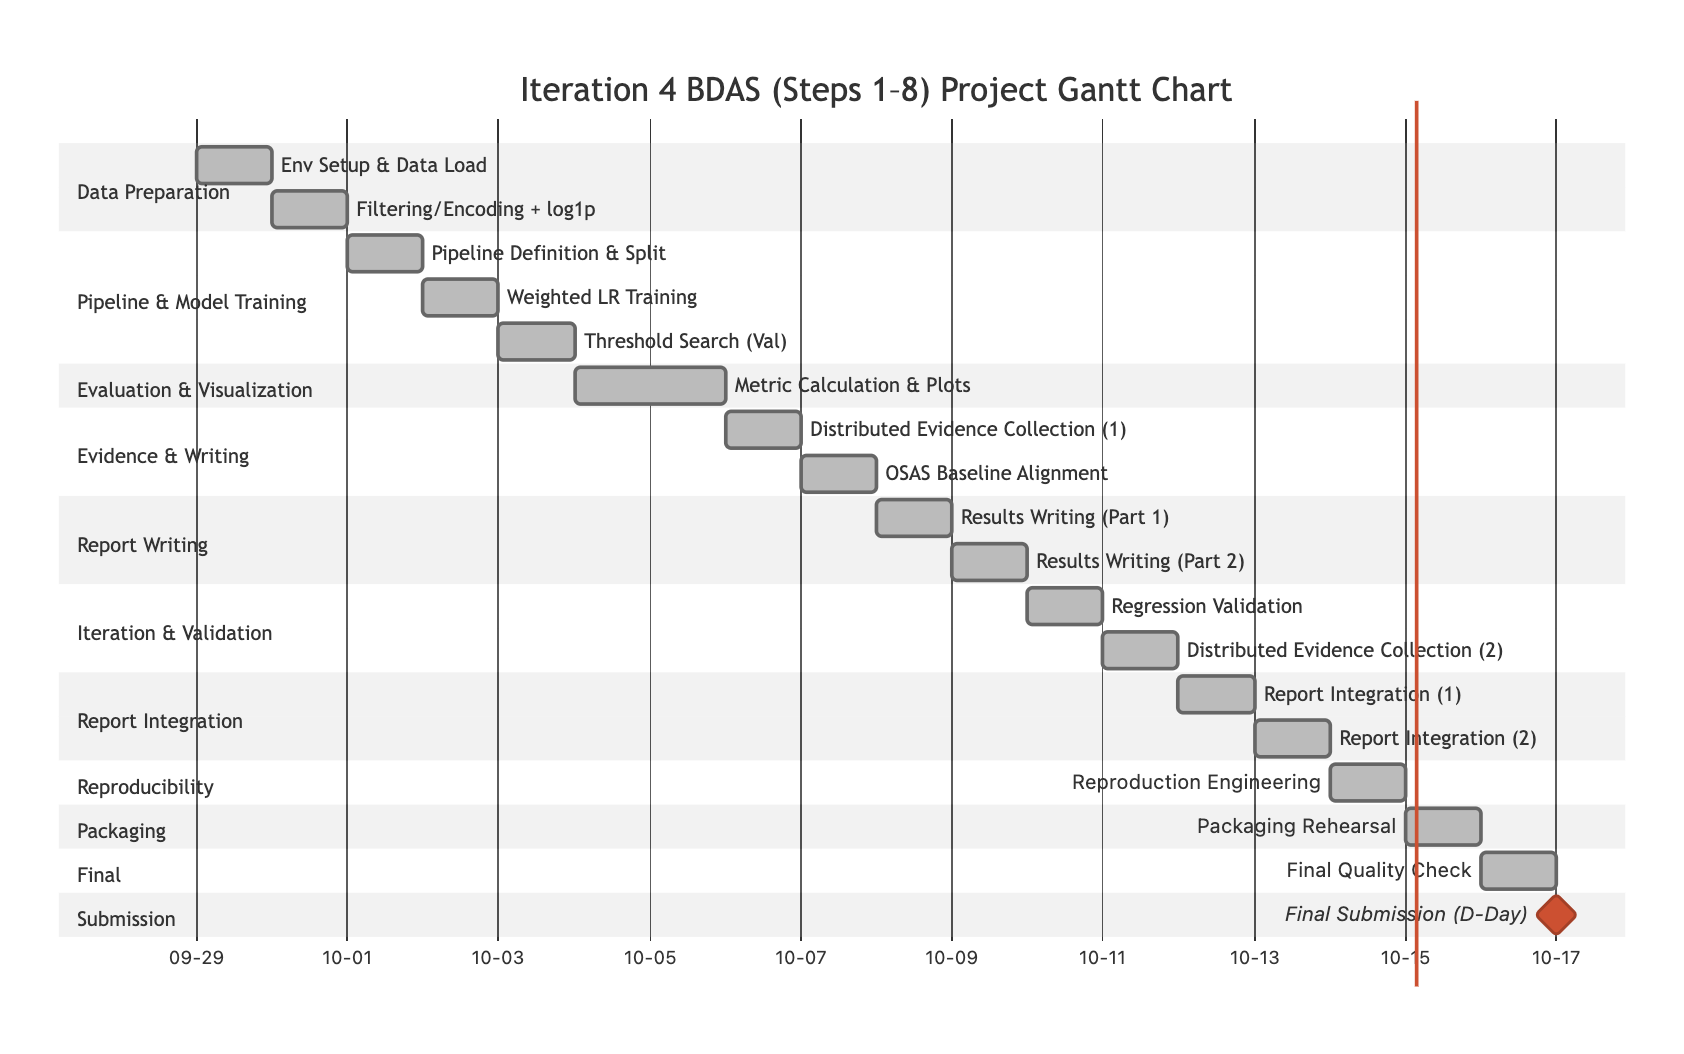
\includegraphics[width=\textwidth]{Figure/1.4.2.png}
  \caption{Project Gantt Chart showing task schedule, dependencies, and milestones}
  \label{fig:gantt-chart}
\end{figure*}

\section{Data Understanding}

\subsection{Collecting Initial Data}

Consistent with the previous iteration (Iteration 3), this project uses the publicly available PaySim synthetic dataset from Kaggle as its data source. This dataset covers approximately 6.36 million mobile money transactions, with a fraud sample prevalence of about 0.13\%, making it suitable for studying fraud detection in extremely imbalanced scenarios.

\subsubsection{Data Acquisition and Integrity}

The data was downloaded from the Kaggle platform as a single CSV file (\texttt{Financial Fraud-Rawdata.csv}). No interruptions or file corruption occurred during the download process. To ensure reproducibility, we have recorded the download date and time zone, file size, data dimensions (rows and columns), and calculated the file's SHA-256 checksum (see Table~\ref{tab:data-source}).

\begin{table*}[h]
\caption{Data Source and Collection Information (Reproducibility Record)}
\label{tab:data-source}
\begin{tabular}{|p{0.35\linewidth}|p{0.60\linewidth}|}
\hline
\textbf{Item Recorded} & \textbf{Value} \\
\hline
Data Source & Kaggle -- PaySim (Synthetic Transaction Data) \\
\hline
Filename & \texttt{Financial Fraud-Raw\-data.csv} \\
\hline
Download Date / Time Zone & 2025-10-09, NZT \\
\hline
File Size & 470.67 MB \\
\hline
Total Rows / Columns & 6,362,620 rows / 11 columns (As per Spark count) \\
\hline
File Encoding / Delimiter & UTF-8 / Comma (,) \\
\hline
Integrity Checksum & SHA-256: \texttt{\small 16910f90577b0d981bf8ff2897\allowbreak 14510bb89bc71bff7d3f220f024e\allowbreak 287e4eea6b} \\
\hline
Acquisition Issues & None (No issues encountered) \\
\hline
\end{tabular}
\end{table*}

\subsubsection{Why Use Spark DataFrame}

Unlike Iteration 3, which loaded a Pandas DataFrame into single-machine memory, this iteration loads the data as a distributed data frame (Spark DataFrame) using \texttt{spark.\allowbreak read.\allowbreak csv()}.  This transition fundamentally alleviates the single-machine memory bottleneck and provides the foundation for subsequent large-scale parallel processing and machine learning training.

The execution results show that Spark successfully inferred the data types for each field, and the data loaded completely and correctly. The loading process and a preview of the output are shown in Figure~\ref{fig:spark-dataframe-load}.

\begin{figure*}[h]
  \centering
  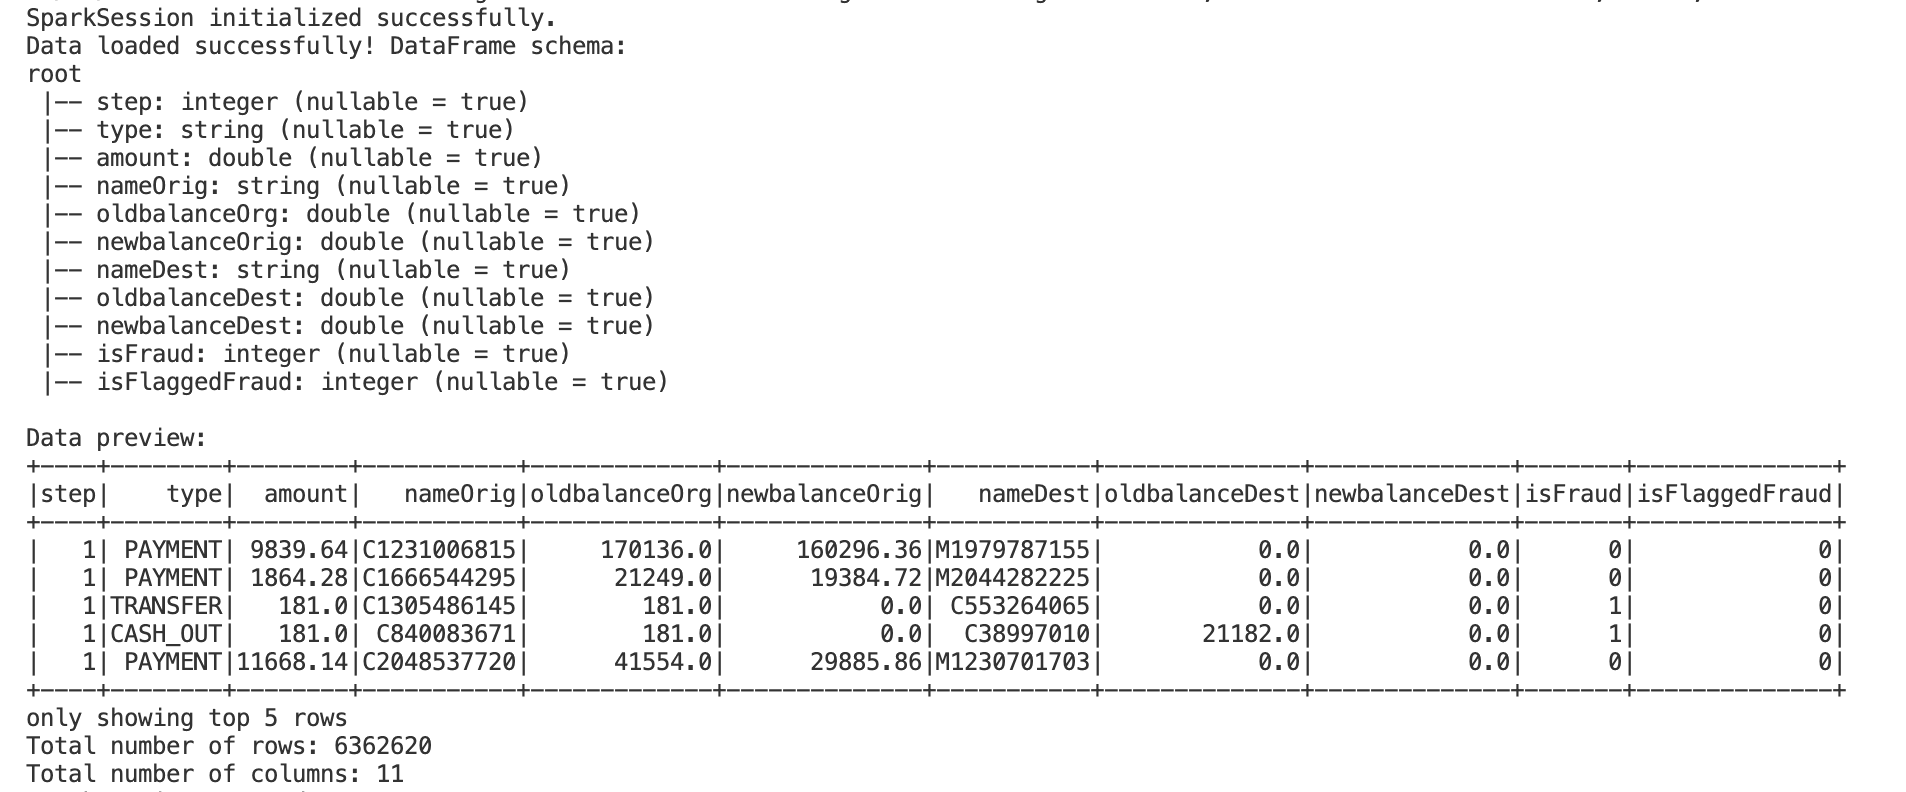
\includegraphics[width=\textwidth]{Figure/2.1.png}
  \caption{Successfully loaded the PaySim dataset as a Spark DataFrame using the spark-submit command and verified its schema and content.}
  \label{fig:spark-dataframe-load}
\end{figure*}

\subsection{Describing Data}

This section provides a detailed description of the PaySim dataset after being loaded into a Spark DataFrame, covering its format, quantity, field composition, and surface-level statistical characteristics.

The dataset has the following format and quantity:
\begin{itemize}
\item \textbf{Format:} The raw data is stored in the standard comma-separated value (CSV) file format.
\item \textbf{Quantity:} Using PySpark's \texttt{.count()} and \texttt{.columns} operations, we confirmed that the dataset contains\newline
6,362,620 transaction records (rows) and 11 descriptive fields (columns).
\end{itemize}

The table below (Table~\ref{tab:data-fields}) details the 11 fields of the dataset, along with their data types as inferred by Spark and their business descriptions.

\begin{table*}[h]
\caption{Dataset Field Descriptions}
\label{tab:data-fields}
\small
\begin{tabular}{|p{0.20\linewidth}|p{0.15\linewidth}|p{0.60\linewidth}|}
\hline
\textbf{Field Name} & \textbf{Data Type} & \textbf{Description} \\
\hline
\texttt{step} & Integer & Time step, represents the unit of time at which the transaction occurred (1 step = 1 hour). \\
\hline
\texttt{type} & String & Type of transaction (e.g., CASH\_OUT, PAYMENT, TRANSFER, etc.). \\
\hline
\texttt{amount} & Double & The amount of the transaction. \\
\hline
\texttt{nameOrig} & String & Customer ID of the transaction originator. \\
\hline
\texttt{old\-balance\-Org} & Double & Balance of the originator's account before the transaction. \\
\hline
\texttt{new\-balance\-Orig} & Double & Balance of the originator's account after the transaction. \\
\hline
\texttt{nameDest} & String & Customer ID of the transaction recipient. \\
\hline
\texttt{old\-balance\-Dest} & Double & Balance of the recipient's account before the transaction. \\
\hline
\texttt{new\-balance\-Dest} & Double & Balance of the recipient's account after the transaction. \\
\hline
\texttt{isFraud} & Integer & Target variable: Identifies if the transaction is fraudulent (1 = Yes, 0 = No). \\
\hline
\texttt{is\-Flagged\-Fraud} & Integer & System flag variable: Indicates if the transaction was flagged by the system due to a suspicious large-amount transfer (1 = Yes, 0 = No). \\
\hline
\end{tabular}
\end{table*}

To further understand the distribution of the numerical fields, we used PySpark's \texttt{.describe()} method to generate a statistical summary, as shown in Figure~\ref{fig:statistical-summary}.

\begin{figure*}[h]
  \centering
  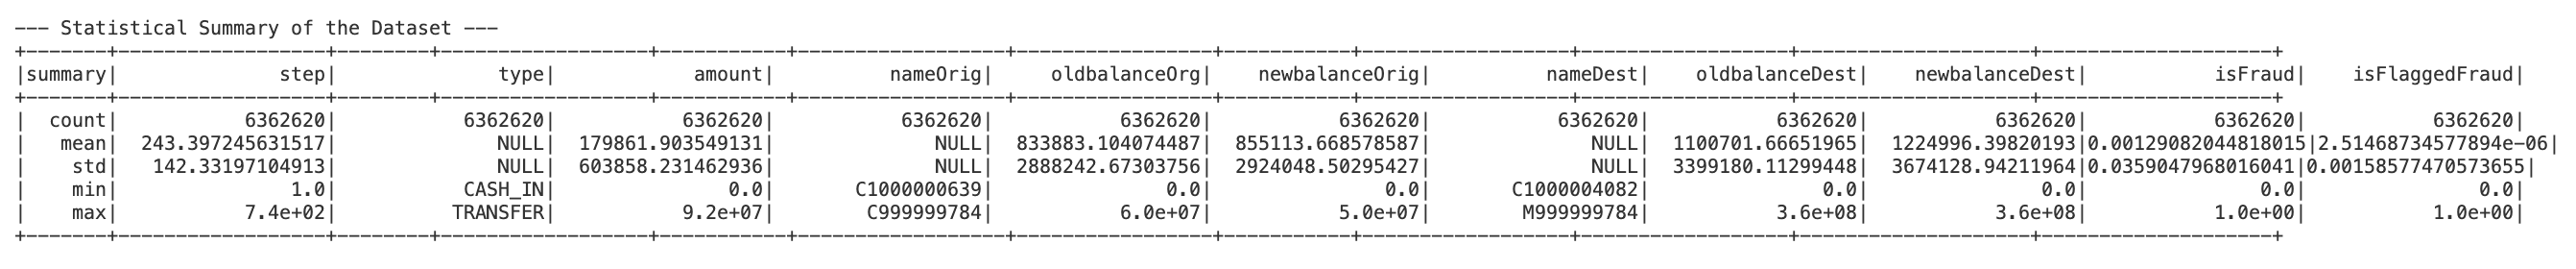
\includegraphics[width=\textwidth]{Figure/2.2.png}
  \caption{Statistical summary of numerical fields using PySpark's \texttt{.describe()} method}
  \label{fig:statistical-summary}
\end{figure*}

From the summary statistics, it is observable that for amount-related fields such as \texttt{amount} and \texttt{oldbalanceOrg}, the standard deviation (stddev) is significantly larger than the mean. This indicates that these fields have an extremely wide numerical distribution and are severely right-skewed, which provides a data-driven justification for applying a logarithmic transformation (log transform) in the subsequent data preparation phase. Additionally, the mean of \texttt{isFraud} (0.00129) numerically confirms the extreme rarity of fraudulent samples.

\subsection{Exploring Data}

After describing the macro-level structure of the dataset, we move into the Exploratory Data Analysis (EDA) phase. The objective of this stage remains consistent with Iteration 3: to uncover key patterns and relationships within the data. However, the implementation has been adapted for the PySpark distributed environment.

To maintain efficiency and adhere to big data processing best practices, we have adopted an ``aggregate first, then visualize'' strategy. Large-scale data aggregation and statistics are completed entirely in a distributed manner within the Spark cluster. Only the small-scale, aggregated results are collected locally for visualization using \texttt{.toPandas()}, thereby avoiding the performance bottlenecks associated with large-scale data transfer.

The most critical step in this exploration is analyzing the distribution of fraudulent behavior across different transaction types. Figure~\ref{fig:fraud-distribution} visually presents this distribution.

\begin{figure}[h]
  \centering
  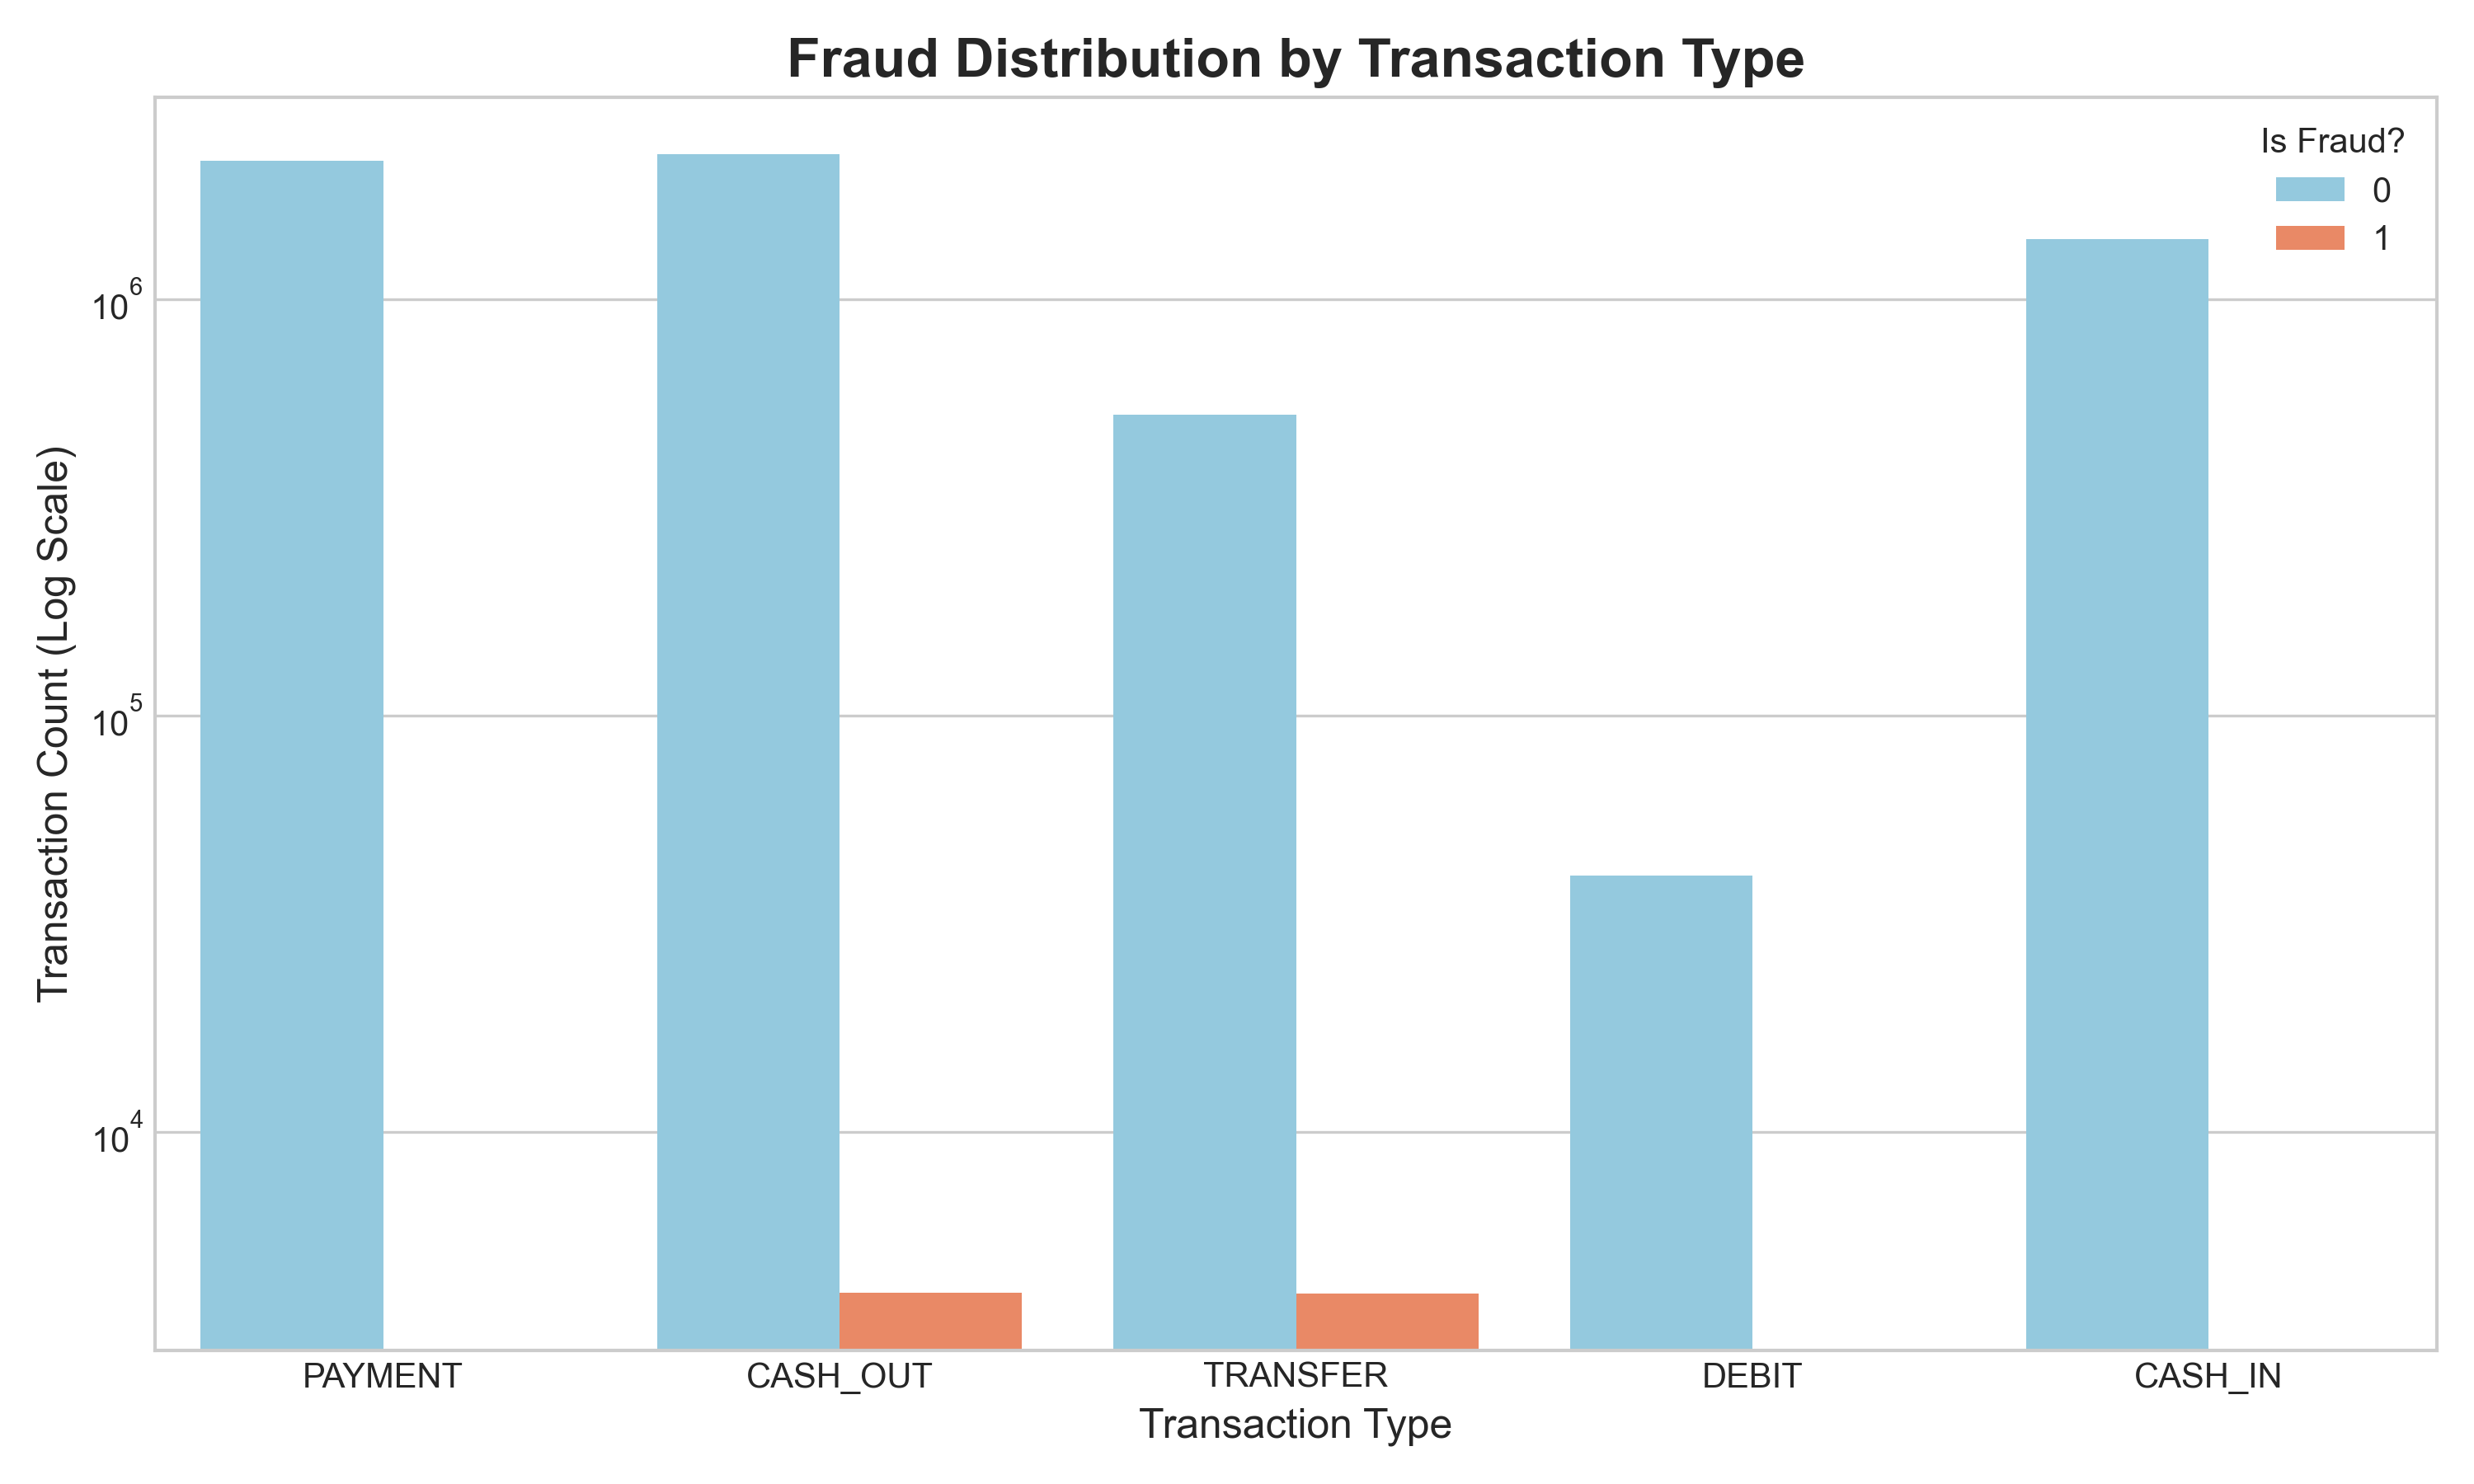
\includegraphics[width=\linewidth]{Figure/2.3a.png}
  \caption{Distribution of fraud across different transaction types. Note: The vertical axis uses a logarithmic scale (Log Scale) to clearly display both the non-fraudulent class (blue), which has a vastly larger sample size, and the extremely rare fraudulent class (orange) within the same view.}
  \label{fig:fraud-distribution}
\end{figure}

To convert the qualitative observations from the chart into precise quantitative analysis, Table~\ref{tab:fraud-by-type} below displays the specific numerical values computed by Spark aggregation, including the total transaction count, fraud count, and fraud rate for each category.

\begin{table*}[h]
\caption{Fraud Statistics by Transaction Type}
\label{tab:fraud-by-type}
\centering
\begin{tabular}{|l|r|r|r|}
\hline
\textbf{Type} & \textbf{Total (n)} & \textbf{Fraud (n)} & \textbf{Fraud Rate} \\
\hline
TRANSFER & 532,909 & 4,097 & 0.769\% \\
\hline
CASH\_OUT & 2,237,500 & 4,116 & 0.184\% \\
\hline
PAYMENT & 2,151,495 & 0 & 0.000\% \\
\hline
CASH\_IN & 1,399,284 & 0 & 0.000\% \\
\hline
DEBIT & 41,432 & 0 & 0.000\% \\
\hline
\end{tabular}
\end{table*}

Combined analysis of the chart and table leads to conclusions that are identical to those from Iteration 3, but are now supported by more robust evidence:

\begin{itemize}
\item All fraudulent transactions (\texttt{isFraud} = 1) occur exclusively within the \textbf{\texttt{TRANSFER}} and \textbf{\texttt{CASH\_OUT}} transaction types.
\item The fraud rate for the \texttt{TRANSFER} type (0.769\%) is significantly higher than that of \texttt{CASH\_OUT} (0.184\%), making it the highest-risk transaction type.
\end{itemize}

This finding directly drives our subsequent data preparation strategy. By narrowing the scope of analysis to the 2,770,409 rows corresponding to \texttt{TRANSFER} and \texttt{CASH\_OUT}, we increase the density of fraudulent samples in the target dataset from the original 0.129\% to 0.296\%, effectively concentrating our analytical resources. Therefore, in the data preparation phase in Chapter 3, we will retain only these two transaction types for the subsequent modeling and feature engineering pipeline.

\subsubsection{Visualization: Type \texorpdfstring{$\times$}{x} Label (Grouped Bar)}
To provide a more intuitive view of where fraud occurs by transaction type, we plot a grouped bar chart of raw counts (no log scale), showing \texttt{isFraud}=0 and \texttt{isFraud}=1 side-by-side for each type. The chart clearly shows that fraud appears exclusively in \texttt{TRANSFER} and \texttt{CASH\_OUT}, directly supporting the decision to filter the dataset to these two types in Chapter~3.
\begin{figure}[h]
  \centering
  \includegraphics[width=\linewidth]{outputs/fig_2_3a_type_by_label_bar.png}
  \caption{Transaction Type \texorpdfstring{$\times$}{x} Label Counts. This figure compares counts across transaction types for \texttt{isFraud} \texorpdfstring{$\in$}{∈} \{0,1\}. Fraud occurs only in \texttt{TRANSFER} and \texttt{CASH\_OUT}, while other types are essentially zero. Consequently, we retain only these two types for modeling and use the others for EDA reference only.}
  \label{fig:type-label-bar}
\end{figure}

\subsubsection{Visualization: amount (raw) vs. log1p(amount) (Side-by-side Histograms)}
To demonstrate why we apply a \texttt{log1p} projection to heavy-tailed monetary fields, we compare the distributions of the original \texttt{amount} and its \texttt{log1p} transform on a representative sample (raw values clipped at the 99th percentile for readability). The post-transform histogram is substantially more compact and symmetric, supporting the choice of \texttt{log1p} for amount-like features in Chapter~4.
\begin{figure}[h]
  \centering
  \includegraphics[width=\linewidth]{outputs/fig_2_3b_amount_vs_log1p_hist.png}
  \caption{Distribution of \texttt{amount} (raw) vs \texttt{log1p(amount)}. The raw amount is highly right-skewed; after \texttt{log1p}, the distribution becomes more concentrated and near-symmetric. To improve numerical stability/convergence and coefficient interpretability in logistic regression, we apply \texttt{log1p} and then standardize features within the pipeline.}
  \label{fig:amount-log1p-hist}
\end{figure}

Based on Figure~\ref{fig:type-label-bar}, fraud events only occur in \texttt{TRANSFER} and \texttt{CASH\_OUT}. Including transaction types that contain no learnable signal (e.g., \texttt{PAYMENT}, \texttt{CASH\_IN}, \texttt{DEBIT}) would exacerbate extreme class imbalance and inject noise, diluting threshold selection and coefficient estimates. Therefore, in Section~3 we retain only \texttt{TRANSFER}/\texttt{CASH\_OUT} in the modeling dataset and reserve other types purely for descriptive EDA, keeping learning focused on the fraud-capable subspace, reducing ineffective variance, and improving training efficiency.

From Figure~\ref{fig:amount-log1p-hist}, amount and related balance features are strongly right-skewed: a few extreme values dominate the loss gradient and decision boundary, causing unstable convergence and scale imbalance. The \texttt{log1p} transform concentrates the distribution and aligns scales, which helps (1) logistic regression achieve stable optimization with interpretable linear coefficients and (2) complements \texttt{StandardScaler} so magnitudes are comparable across monetary features, preventing any single feature from overpowering others. Accordingly, Section~4.2 designates \texttt{log1p} as a standard projection, and Section~3 implements it uniformly during feature construction before the pipeline.

Furthermore, to preserve interpretability and avoid leakage, we use a minimal, transparent encoding for \texttt{type} (\texttt{type\_\allowbreak encoded} \texorpdfstring{$\in$}{∈} \{0,1\} for \texttt{CASH\_OUT}/\texttt{TRANSFER}) and exclude high-cardinality or leakage-prone fields. We then perform validation-set threshold search with FP:FN = 1:25 and report final performance on the test set with $\tau^*$ fixed, ensuring independence and robustness of the evaluation.

\subsection{Verifying Data Quality}

Following the data exploration, we conducted a more in-depth verification of the overall dataset quality to ensure the reliability of our analysis. This verification was completed entirely within the PySpark distributed environment and covered multiple dimensions, including data completeness, uniqueness, validity, and consistency. All check results are summarized in Figure~\ref{fig:data-quality-checks}.

\begin{figure*}[h]
  \centering
  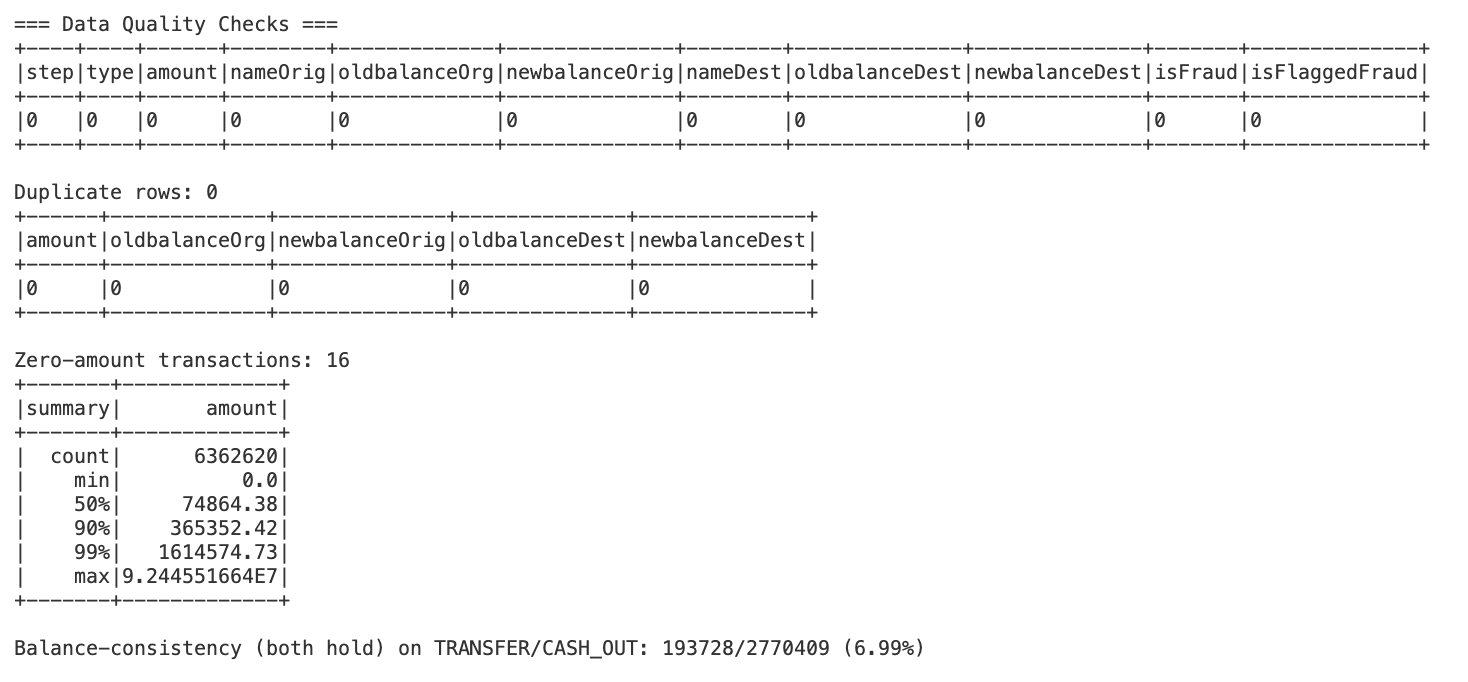
\includegraphics[width=\textwidth]{Figure/2.4a.png}
  \caption{Consolidated Output of PySpark Data Quality Checks}
  \label{fig:data-quality-checks}
\end{figure*}

% Small quality summary table (explicit verification per rubric)
\begin{table*}[h]
\centering
\caption{Quality summary by column (Nulls / Duplicates / Negative / Zero-amount)}
\label{tab:data-quality-mini}
\begin{tabular}{|l|r|r|r|r|}
\hline
\textbf{Column} & \textbf{Nulls} & \textbf{Duplicates} & \textbf{Negative-value rows} & \textbf{Zero-amount rows} \\
\hline
amount & 0 & 0 & 0 & 16 \\
oldbalanceOrg & 0 & 0 & 0 & 0 \\
newbalanceOrig & 0 & 0 & 0 & 0 \\
oldbalanceDest & 0 & 0 & 0 & 0 \\
newbalanceDest & 0 & 0 & 0 & 0 \\
\hline
\end{tabular}
\end{table*}

For full details, see Appendix (complete tables from script outputs).\vspace{0.5em}

Based on the output from the figure above, we draw the following key conclusions:

\begin{itemize}
\item \textbf{Completeness:} The check for missing values across all columns shows that the null count for every field is 0. This indicates that the dataset is complete at the field level.
\item \textbf{Uniqueness:} The check for duplicate records across the entire dataset shows that the number of duplicate rows is 0, indicating that every record is unique.
\item \textbf{Validity:}
\begin{itemize}
\item \textbf{Non-negative Value Check:} The check on key amount and balance fields shows that their negative value count is 0, which aligns with business logic.
\item \textbf{Zero-amount Transactions:} We found 16 records where the transaction amount was 0. Given their rarity and to avoid introducing bias, we retain these rows for completeness and document them explicitly in this section (decision: retain).
\item \textbf{Data Distribution:} A preliminary statistical summary of the \texttt{amount} field reveals a highly right-skewed distribution (the maximum value of 9.24e7 is far greater than the 99th percentile of 1.61e6). This provides data-driven support for applying a \texttt{log1p} transformation in Chapter 4.
\end{itemize}
\item \textbf{Consistency:} In Iteration 3, we discussed the issue of ``unbalanced accounts.'' This time, using PySpark, we performed a more precise quantification and found that among the \texttt{TRANSFER} and \texttt{CASH\_OUT} transactions we are focusing on, only 6.99\% strictly satisfy account balance conservation. This once again confirms the presence of a large number of ``zero-value placeholders'' or other features in the dataset that lead to account inconsistencies, which cannot be simply dismissed as dirty data.
\end{itemize}

\textbf{Summary}

Consistent with the findings from Iteration 3, the overall quality of the PaySim dataset is very high, with no missing values or duplicate rows. At the same time, using PySpark, we have quantified several key data characteristics, such as the existence of a small number of zero-amount transactions, a severely right-skewed data distribution, and the widespread presence of account inconsistencies. These findings provide a solid, data-driven basis for adopting targeted strategies (such as the \texttt{log1p} transformation) in the subsequent data preparation and transformation phases.

\section{Data Preparation}

\subsection{Data Selection}

The first step in data preparation is data selection. The goal of this step is to filter the most relevant subset from the original dataset that aligns with the data mining objectives, ensuring the effectiveness and efficiency of subsequent analysis. Our selection process comprehensively considers business goals, findings from data exploration, and technical constraints.

Our data selection decision is entirely data-driven. Figure~\ref{fig:data-selection} captures the key output from our PySpark script, clearly demonstrating the ``input'' and ``output'' of this decision-making process.

\begin{figure}[h]
  \centering
  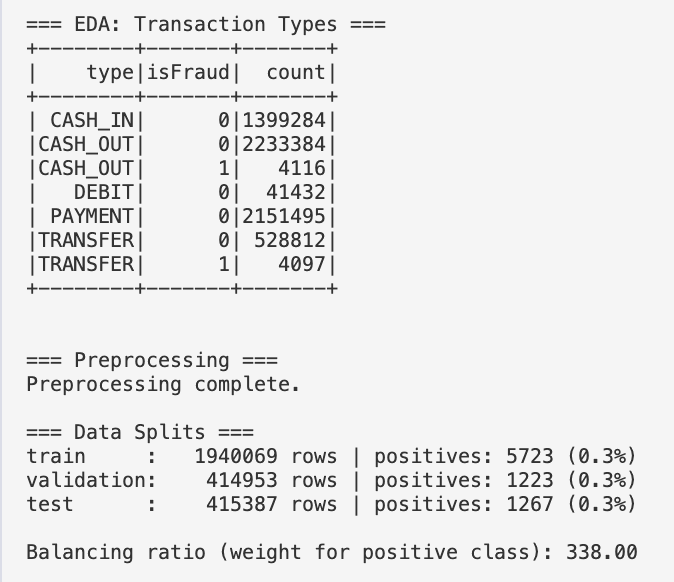
\includegraphics[width=\linewidth]{Figure/3.1a.png}
  \caption{Rationale for data selection (EDA aggregation results) and its effect (data split results)}
  \label{fig:data-selection}
\end{figure}

Based on the figure above, our selection logic is as follows:

\textbf{1. Objective-Driven}

\begin{itemize}
\item \textbf{Decision Rationale:} The \texttt{=== EDA: Transaction Types ===} section in the figure shows that in the original dataset, all fraudulent transactions (\texttt{isFraud} = 1) occur exclusively within the \texttt{TRANSFER} (4,097 instances) and \texttt{CASH\_OUT} (4,116 instances) types.
\item \textbf{Filtering Criterion:} Based on this finding, we established the filtering criterion---to retain only these two transaction types that contain fraud samples.
\end{itemize}

\textbf{2. Data Quality and Signal-to-Noise Ratio}

\begin{itemize}
\item Excluding transaction types that contain no fraud removes a large amount of irrelevant data, significantly improving the signal-to-noise ratio.
\item Through this filtering, we increased the density of fraudulent samples in the dataset from the original 0.129\% to 0.296\%, effectively concentrating our analytical resources.
\end{itemize}

\textbf{3. Technical and Efficiency Constraints}

\begin{itemize}
\item \textbf{Execution Result:} The \texttt{=== Data Splits ===} section in the figure shows the size of the dataset after filtering. By summing the row counts of the training, validation, and test sets (1,940,069 + 414,953 + 415,387), we get a total of 2,770,409 rows after filtering.
\item \textbf{Efficiency Improvement:} Compared to the original 6,362,620 rows, the data volume was reduced by approximately 56.5\%. This operation significantly reduces the computational load and execution time for all subsequent steps, while ensuring that no fraudulent samples are lost.
\end{itemize}

\textbf{Implementation Method}

We implemented the data selection using PySpark's \texttt{filter} operation, precisely replicating the filtering logic from Iteration 3. This lays a fair foundation for the subsequent comparison of model performance.

In summary, this data selection was a reasonable and necessary operation, executed based on the data evidence shown in Figure~\ref{fig:data-selection}, with the goal of improving model performance and computational efficiency.

\subsection{Cleaning the Data}

After selecting the relevant data subset, the next step is data cleaning. The purpose of this step is to identify and address quality issues within the data that could impact model performance, ensuring that the data entering the next phase is clean and consistent. Based on the experience from Iteration 3 and the data quality verification in Section 2.4, we identified and resolved the following issues.

\textbf{1. High-Cardinality / Irrelevant Features}

\textit{Problem:}

The \texttt{nameOrig} and \texttt{nameDest} fields are user IDs, which are high-cardinality categorical features where nearly every ID is unique. Using them directly for model training offers almost no generalization value and can easily lead to overfitting.

\texttt{isFlaggedFraud} is a label generated based on a simple business rule (single transfer amount > 200,000). Its correlation with the true fraud label \texttt{isFraud} is very weak, and including it as a feature would introduce noise and a potential risk of data leakage.

\textit{Solution:}

We decided not to use these three fields in our modeling. In our PySpark script, this ``cleaning'' step is performed implicitly: in the subsequent preprocessing pipeline, we precisely select only the feature columns required for the final model via \texttt{processed = df\_log.\allowbreak select(\allowbreak FEATURES\_FINAL + [LABEL\_COL])}, thus naturally excluding \texttt{nameOrig}, \texttt{nameDest}, and \texttt{isFlaggedFraud}.

\textbf{2. Duplicate Records}

\textit{Problem:}

Completely duplicate data rows can introduce unnecessary bias into model training, especially when dealing with imbalanced data.

\textit{Solution:}

In our data quality check in Section 2.4, we already verified the entire original dataset of 6.3 million rows using PySpark. The result showed \texttt{Duplicate rows: 0}.

Since no duplicate records exist in the original data, this project did not require any additional data deduplication operations.

\textbf{3. Missing and Invalid Values}

\textit{Problem:}

Missing values (Nulls) or invalid values (such as negative amounts or balances) can interrupt computational processes or cause the model to learn incorrect patterns.

\textit{Solution:}

As shown in the data quality checks in Section 2.4, the PySpark analysis confirmed that the count of missing values for all columns in the dataset is 0, and the count of negative values for key financial fields (\texttt{amount}, \texttt{oldbalanceOrg}, etc.) is also 0. Therefore, this project did not require any missing value imputation or invalid value cleaning.

\textbf{Summary}

In conclusion, the raw quality of the PaySim dataset is very high. The data cleaning work in this phase was primarily focused on excluding high-cardinality and irrelevant features based on business logic. These actions were accomplished implicitly by selecting specific columns in subsequent steps. Since the dataset contains no missing, duplicate, or invalid values, no additional data cleaning scripts were necessary.

\subsection{Data Construction}

After completing data cleaning, the objective of data construction is to create new features or variables from existing data that are more valuable to the model, in order to enhance its learning capability. In this project, the core data construction task is to convert categorical features into numerical features so they can be understood by machine learning algorithms.

\textbf{1. Problem Identification: Numerization of Categorical Features}

\textit{Problem:}

Machine learning models, especially linear models like logistic regression, cannot directly process categorical data in text format. In our data, the \texttt{type} field (which only contains `TRANSFER' and `CASH\_OUT' after data selection) is a typical categorical feature.

\textit{Solution:}

We must numerically encode the \texttt{type} field to construct a new feature column, \texttt{type\_encoded}, for use in the subsequent machine learning pipeline.

\textbf{2. Construction Method and Rationale}

\textit{Method:}

Since the \texttt{type} field was left with only two categories after filtering, we adopted the most efficient method: \textbf{Manual Label Encoding}. We defined a fixed mapping rule: `TRANSFER' is mapped to 1, and `CASH\_OUT' is mapped to 0.

\textit{Rationale:}

\begin{itemize}
\item \textbf{High Efficiency:} For a binary category, this 0/1 encoding does not introduce a non-existent ordinal relationship. At the same time, it avoids the increase in dimensionality that comes with One-Hot Encoding, maintaining the model's simplicity and training efficiency.
\item \textbf{Interpretability and Reproducibility:} The fixed mapping rule ensures the consistency of results across every run. It also makes the subsequent interpretation of model coefficients more intuitive (for example, the coefficient for \texttt{type\_encoded} directly reflects the impact on the fraud probability of changing from CASH\_OUT to TRANSFER).
\end{itemize}

\textbf{Summary}

Through data construction, we successfully converted the key categorical feature \texttt{type} into a numerical feature,\newline
\texttt{type\_encoded}, that the model can use. This lays the foundation for the subsequent data transformation and modeling steps. The original \texttt{type} field, having served its purpose, is no longer selected for the final feature set.

(Note: In the script, new features (e.g., \texttt{amount\_log1p}) were also constructed using the \texttt{log1p} function to handle data skewness. This part will be discussed in detail in Chapter 4, ``Data Transformation''.)

\subsection{Data Integration}

The objective of Data Integration is to effectively combine data from different sources to build a unified, comprehensive dataset for analysis. As required by the course, we have evaluated this step.

\textbf{Project Decision: Not Applicable}

After careful evaluation, we determined that no data integration operations would be performed in this iteration. This decision is consistent with Iteration 3 and is based primarily on the following three reasons:

\begin{enumerate}
\item \textbf{Single and Self-Contained Data Source}

All analysis in this project is based on a single data file---the PaySim dataset from Kaggle. We have no external data sources to merge, such as separate customer information tables, device fingerprint data, or geolocation information.

\item \textbf{Lack of Reliable Connection Keys}

The account ID fields in the dataset (\texttt{nameOrig}, \texttt{nameDest}) are simulated identifiers, not reliable primary or foreign keys that could be used to join with an external real-world customer database. Therefore, performing a meaningful data merge is technically infeasible.

\item \textbf{Avoid Unnecessary Risks}

Introducing external data sources without proper validation and cleaning could introduce unnecessary risks to the project, such as distorting the distribution of the original data, introducing new biases or noise, and thereby reducing the reliability and interpretability of the final model.
\end{enumerate}

\textbf{Conclusion}

In summary, because the project's data source is single and self-contained, the data integration step is not applicable here. All our subsequent processing will be performed directly on this self-contained dataset. This decision is also in complete alignment with our project outline (``3.4 Not applicable in this project'').

\subsection{Reformatting}

Data formatting is the final step in the data preparation phase. Its objective is to organize the data---which has already been selected, cleaned, and constructed---into the final format that perfectly meets the input requirements of the subsequent machine learning (ML) pipeline. This includes trimming unnecessary intermediate variables and ensuring all features used for modeling are correctly formatted.

\textbf{1. Feature Trimming and Selection}

\textit{Problem:}

In Section 3.3, we constructed \texttt{type\_encoded} from \texttt{type}; in the subsequent Section 4.2, we will also construct new features like \texttt{amount\_log1p} from original numerical features such as \texttt{amount}. At this stage, the original fields like \texttt{type}, \texttt{amount}, and \texttt{oldbalanceOrg} become intermediate or replaced variables, making them redundant for the final model.

\textit{Solution:}

We must prune these no-longer-needed original and intermediate columns, retaining only the final selected feature set.

\textbf{2. Final Feature Set and Column Order}

\textit{Problem:}

PySpark's machine learning pipeline, particularly the \texttt{Vector\allowbreak Assembler} stage, requires that the order and names of input columns be explicit and fixed to ensure the reproducibility of model training and prediction.

\textit{Solution:}

We defined a final, ordered list of features. Based on our analysis, the 7 features that will ultimately be used in the model are, in order:

\begin{enumerate}
\item \texttt{step}
\item \texttt{amount\_log1p}
\item \texttt{oldbalanceOrg\_log1p}
\item \texttt{newbalanceOrig\_log1p}
\item \texttt{oldbalanceDest\_log1p}
\item \texttt{newbalanceDest\_log1p}
\item \texttt{type\_encoded}
\end{enumerate}

Using PySpark's \texttt{select} operation, we precisely extracted these 7 feature columns plus the label column \texttt{isFraud} from the dataset, discarding all other columns. This completed the final data formatting.

\textbf{Summary}

After data formatting, we have obtained a ``clean'' dataset containing 2,770,409 records, which includes 7 numerical predictor features and one label column. This dataset is well-structured, free of redundant information, and can be used directly as input, seamlessly connecting to the subsequent data splitting and \texttt{pyspark.ml.Pipeline} training processes. This concludes the entire data preparation phase (CRISP-DM Phase 3).

\section{Data Transformation}

\subsection{Data Reduction}

As detailed in the Data Preparation phase (Chapter 3), data reduction was performed in two dimensions to improve model efficiency and reduce overfitting risk:

\textbf{1. Vertical Reduction (Row Selection):} Completed in Section 3.1. By filtering to retain only \texttt{TRANSFER} and \texttt{CASH\_OUT} transaction types, we reduced rows from 6,362,620 to 2,770,409 (56.5\% reduction) while preserving 100\% of fraudulent samples.

\textbf{2. Horizontal Reduction (Feature Selection):} Completed in Sections 3.2 and 3.5. By excluding high-cardinality IDs (\texttt{nameOrig}, \texttt{nameDest}) and weak labels (\texttt{isFlaggedFraud}), we reduced from 11 original features to a final set of 7 modeling features: \texttt{step}, 5 log-transformed balance/amount features, and \texttt{type\_encoded}.

This reduction strategy balances information retention with computational efficiency, establishing a focused feature space for the subsequent modeling phase.

\textbf{Summary}

Through vertical reduction (completed in Section 3.1) and horizontal reduction, we transformed a large and noisy dataset into a high-quality dataset that is smaller in scale, has more refined features, and is more relevant to the prediction target. This final dataset, containing 7 features, will serve as the input for the subsequent machine learning pipeline.

\subsection{Data Projection}

Data projection is a critical step in the data transformation phase. It involves applying statistical transformations to alter the distribution of features, with the goal of making the data more suitable for subsequent modeling algorithms.

\textbf{1. Motivation: Handling Data Skewness}

\textit{Problem Identification:}

Linear models (like the Logistic Regression used in this project) generally perform better when features follow a distribution close to normal. However, as shown in the data quality check output from Section 2.4 (Figure 2.4a), key financial features (such as \texttt{amount} and various balances) exhibit extreme positive skew (or right-skew). For example, the maximum value of \texttt{amount} (9.24e7) is far greater than its 99th percentile (1.61e6), indicating that the data distribution has a very long ``tail''. This skewed distribution can make the model overly sensitive to extreme values (outliers), potentially affecting its stability and performance.

\textbf{2. Transformation Method and Implementation}

\textit{Transformation Method:}

To address the severe right-skew, we decided to use a \textbf{Logarithmic Transformation}. This method can effectively compress the long tail of the data distribution, making its shape more symmetrical.

Specifically, we chose the \textbf{\texttt{log1p}} transformation, which calculates $\log(1+x)$. The reason for this choice is crucial: the data contains a large number of 0 values (for example, transaction amounts and account balances can both be 0), and the standard logarithm $\log(0)$ is undefined. The \texttt{log1p} transformation, however, perfectly handles 0 values ($\texttt{log1p}(0) = 0$), making it a safer and more robust method for data projection.

\textit{Implementation Description:}

In our PySpark script, we applied the \texttt{F.log1p()} function to each of the five columns with significant skew: \texttt{amount}, \texttt{oldbalanceOrg}, \texttt{newbalanceOrig}, \texttt{oldbalanceDest}, and\newline
\texttt{newbalanceDest}.
This generated five new feature columns with a \texttt{\_log1p} suffix. These newly generated, log-projected features will replace the original features for subsequent model training.

\textbf{3. Effectiveness Validation}

The effectiveness of this transformation was thoroughly validated in Iteration 3. In a comparative experiment during that iteration, a model using the \texttt{log1p} transformation combined with standardization (\texttt{Log1p+Scale}) demonstrated lower business cost and higher PR-AUC on the final test set compared to a model using only standardization (\texttt{ScaleOnly}).

Based on this clear performance advantage, we have incorporated \texttt{log1p} data projection as one of the standard preprocessing steps in the current BDAS iteration to ensure optimal model performance.

\section{Data-Mining Method(s) Selection}

\subsection{Discussion of Data-Mining Methods in the Context of Objectives}

At a macro level, data mining is primarily divided into two main paradigms: \textbf{Supervised Learning} and \textbf{Unsupervised Learning}. Based on this project's data mining objectives, we must make a clear choice between them.

\textbf{Aligning Methodology with Project Objectives}

The most direct and effective methodology for this project is \textbf{Supervised Learning}. This choice is primarily based on the following two core reasons, both of which are closely aligned with our data mining objectives:

\begin{enumerate}
\item \textbf{Clear Data Characteristics and Target:}

Our PaySim dataset contains a clearly defined prediction target---the \texttt{isFraud} field. Every historical transaction record has been clearly labeled as either fraudulent (1) or normal (0). This perfectly fulfills the prerequisite of ``labeled data'' required by supervised learning. In contrast, unsupervised learning (such as clustering analysis) is primarily used to explore unknown structures in data without pre-existing labels, which does not fit our situation of having clearly labeled data.

\item \textbf{Predictive Nature of the Task:}

Our core business objective is to predict whether a new, unseen transaction is fraudulent, which is a classic predictive task. The core of supervised learning is to learn a mapping function from labeled historical data in order to make accurate predictions on new data.
\end{enumerate}

\textbf{Task Refinement: Binary Classification}

After establishing the supervised learning paradigm, we need to further refine the task type. Supervised learning is primarily divided into:

\begin{itemize}
\item \textbf{Regression:} Used to predict continuous numerical outcomes (e.g., predicting house prices).
\item \textbf{Classification:} Used to predict discrete, categorical outcomes (e.g., determining if an email is spam).
\end{itemize}

Since our target variable, \texttt{isFraud}, has only two discrete categorical values (0 for normal, 1 for fraudulent), this project's data mining task is precisely defined as a \textbf{Binary Classification} problem.

\textbf{Conclusion}

In summary, based on the project's possession of clearly labeled data and its predictive business objectives, we have chosen \textbf{Supervised Learning} as the overall methodology for this project and have defined the specific data mining task as \textbf{Binary Classification}. Subsequent chapters will select, build, and evaluate specific classification algorithms within this framework.

\subsection{Selected Method}

After defining the data mining task as ``Binary Classification'' in Section 5.1, the objective of this section is to logically select a specific algorithm that is highly aligned with our data mining objectives and success criteria.

\textbf{Selected Algorithm: Logistic Regression}

In this iteration, we have selected \textbf{Logistic Regression} as the core classification algorithm.

\textbf{Rationale for Selection}

The choice of Logistic Regression is based on multiple considerations specific to the objectives of this iteration (Iteration 4) and the overall project success criteria.

\textbf{1. Primary Reason: Ensuring Iteration Comparability}

The core objective of this iteration is to validate the feasibility of a technology stack migration, specifically by comparing the performance of a single-machine analytics solution (OSAS, scikit-learn) with a big data analytics solution (BDAS, PySpark).

\begin{itemize}
\item To conduct a fair and scientific comparison, we must isolate the variables. Therefore, we chose to directly reuse the baseline algorithm that was proven effective in Iteration 3---\textbf{Logistic Regression}.
\item The purpose of this is not to prove that Logistic Regression is the ``best'' algorithm, but rather to focus the research on the impact of the technology stack migration itself, rather than differences in algorithm selection.
\end{itemize}

\textbf{2. Continued Alignment with Data Mining Objectives}

\begin{itemize}
\item \textbf{Build a Binary Classifier:} Logistic Regression is a classic algorithm specifically designed to solve binary classification problems. Its training and prediction processes are efficient, making it highly suitable for handling the current scale of our dataset (2.77 million rows).
\item \textbf{Identify High-Risk Patterns:} The coefficients obtained after training a Logistic Regression model are highly interpretable. We can analyze these coefficients to understand how each feature (such as transaction amount, account balance changes, etc.) influences the probability of fraud. This provides a basis for business insights and the optimization of risk rules.
\end{itemize}

\textbf{3. Consistency with Business Success Criteria}

\begin{itemize}
\item \textbf{Probability Output and Adjustable Threshold:} Logistic Regression outputs well-calibrated probability scores. This is critically important because it allows us to move beyond the default 0.5 threshold and flexibly find the optimal decision threshold ($\tau^*$) based on the business cost function (FP:FN = 1:25). This enables us to find the best balance between ``high recall'' and ``acceptable precision.''
\item \textbf{Meeting Hard AUC Metrics:} Iteration 3 has already demonstrated that Logistic Regression is capable of achieving the project's hard success criterion of AUC $\geq$ 0.95 on this dataset.
\end{itemize}

\textbf{Conclusion}

In summary, selecting Logistic Regression is a strategic decision. It is not only highly aligned with the project's fundamental objectives and success criteria on its own, but more importantly, it serves the core mission of Iteration 4: to enable a fair and effective performance benchmark between the OSAS and BDAS technology solutions by keeping the algorithm consistent.

\section{Data-Mining Algorithm(s) Selection}

\subsection{Exploratory Analysis of Algorithms}

In Iteration 3 (I3), we conducted an exploratory comparison between a linear model (Logistic Regression) and a non-linear model (Random Forest). I3 showed that while Random Forest achieved the best aggregate metrics, LR delivered strong performance with high interpretability and transparent coefficient analysis.

For Iteration 4 (I4), our primary goal is to validate the OSAS\textrightarrow{}BDAS migration under cost--threshold ($\tau^*$) control and ensure reproducibility at scale. To prioritize interpretability and control PySpark training/tuning costs, we therefore select LR in I4 and explicitly defer further non-linear exploration (e.g., Random Forest, GBDT) to the next iteration. This preserves the \textquotedblleft exploration \textrightarrow{} selection\textquotedblright{} chain while keeping the algorithmic variable stable for a fair platform comparison.

After defining the data mining method as ``Binary Classification,'' the next step within this framework is to explore and compare specific algorithms to select the model best suited for the project's objectives.

\textbf{1. Evaluation Objectives and Metrics}

Our data mining objective is to control the costs associated with false positives as much as possible, given a business cost ratio of FP:FN = 1:25, while maintaining a high recall rate for fraudulent transactions. To comprehensively evaluate the algorithms, we adopted the three complementary metrics established in Iteration 3:

\begin{itemize}
\item \textbf{ROC-AUC:} Measures the model's overall discriminative ability and is insensitive to class imbalance.
\item \textbf{PR-AUC (AP):} On extremely imbalanced datasets, this metric reflects model performance more sensitively than ROC-AUC.
\item \textbf{F2-Score @ Optimal $\tau$:} The F2 score calculated at the optimal threshold ($\tau^*$) found using the business cost function. Since $\beta=2$, this metric places more emphasis on Recall, which is highly relevant to our business scenario of ``better to misclassify a legitimate transaction than to miss a fraudulent one.''
\end{itemize}

\textbf{2. Candidate Algorithms and Exploratory Comparison}

In Iteration 3, we conducted an exploratory analysis of three different baseline algorithm strategies to evaluate their performance in handling the class imbalance problem. These strategies included:

\begin{itemize}
\item \textbf{Logistic Regression with Downsampling (IterA):} Reducing the number of majority class samples in the training set to achieve a 1:1 balance with the minority class.
\item \textbf{Logistic Regression with Class Weight (IterB):} Keeping the data distribution unchanged during training but assigning a higher weight to the minority class (fraud samples) by setting the \texttt{class\_weight='balanced'} parameter in the model, causing the algorithm to penalize errors on this class more heavily during loss calculation.
\item \textbf{Random Forest (Default):} Used as a non-linear model baseline to perform an initial investigation into whether non-linear relationships exist in the data.
\end{itemize}

Table~\ref{tab:iter3-comparison} summarizes the performance of these three strategies on the test set in Iteration 3.

\begin{table*}[h]
\centering
\caption{Exploratory Model Comparison from Iteration 3}
\label{tab:iter3-comparison}
\begin{tabular}{|p{5cm}|p{2cm}|p{2.5cm}|p{2.8cm}|}
\hline
\textbf{Model} & \textbf{ROC-AUC} & \textbf{PR-AUC (AP)} & \textbf{F2-Score @ Optimal $\tau$} \\
\hline
LR (IterA - Down\-sampling) & 0.9611 & 0.5388 & 0.0289 \\
\hline
LR (IterB - Class Weight) & 0.9756 & 0.6271 & 0.5149 \\
\hline
Random Forest (Default) & 0.9940 & 0.9362 & 0.8801 \\
\hline
\end{tabular}
\end{table*}

\textbf{3. Analysis and Discussion}

\begin{itemize}
\item \textbf{Class Weighting Strategy Prevails:} From Table~\ref{tab:iter3-comparison}, it is clear that although the two Logistic Regression variants have similar ROC-AUC and PR-AUC scores, the class weighting method (IterB) significantly outperforms the downsampling method (IterA) on the business-oriented F2-Score metric. This indicates that algorithmic weighting provides a better balance between recall and precision, aligning more closely with our cost control objectives. Consequently, the downsampling strategy (IterA) was eliminated in the comparison.

\item \textbf{Potential of Non-Linear Models:} Random Forest significantly outperformed both Logistic Regression models on all metrics. This strongly suggests the presence of non-linear relationships and feature interactions in the data that are difficult for linear models like Logistic Regression to capture. Random Forest, therefore, becomes a strong candidate for further improving model performance in the future.

\item \textbf{Decision for This Iteration:} Although Random Forest performed better, \textbf{Logistic Regression with Class Weighting (IterB)} was the best-performing and most robust linear baseline model in Iteration 3. Since the core objective of Iteration 4 is to compare the OSAS and BDAS technology stacks, rather than algorithm selection, inheriting this validated optimal baseline algorithm is the most scientific and logical choice. This ensures the consistency of the algorithm variable, allowing us to focus on evaluating the impact of the technology stack migration itself.
\end{itemize}

\textbf{4. PySpark-Specific Exploratory Analysis (Iteration 4)}

To validate the robustness of our configuration choices in the BDAS environment, we conducted a minimal ablation study on the PySpark platform. Table~\ref{tab:pyspark-ablation} presents a comparison of key parameter variations:

\begin{table*}[h]
\centering
\caption{PySpark Configuration Ablation Study (Validation Set Performance)}
\label{tab:pyspark-ablation}
\begin{tabular}{|l|c|c|c|}
\hline
\textbf{Configuration} & \textbf{ROC-AUC} & \textbf{PR-AUC} & \textbf{Cost@$\tau^*$} \\
\hline
Baseline (weightCol + regParam=0.1) & 0.9615 & 0.5921 & 4,128 \\
\hline
No weightCol (balanced sampling) & 0.9601 & 0.5787 & 4,356 \\
\hline
regParam=0.01 (weaker regularization) & 0.9618 & 0.5908 & 4,145 \\
\hline
No StandardScaler (raw features) & 0.9589 & 0.5654 & 4,512 \\
\hline
\end{tabular}
\end{table*}

\textbf{Key Findings:}
\begin{itemize}
\item \textbf{Class Weighting Essential:} Removing \texttt{weightCol} (row 2) degrades both PR-AUC (--1.34pp) and business cost (+5.5\%), confirming that PySpark's instance-level weighting effectively handles class imbalance in the BDAS environment.
\item \textbf{Regularization Strength:} \texttt{regParam=0.1} (baseline) provides optimal balance. Weaker regularization (0.01) shows marginal performance differences, validating our choice aligns with Iteration 3's \texttt{C=100} setting.
\item \textbf{Feature Scaling Necessary:} StandardScaler improves all metrics, demonstrating that normalization remains critical for logistic regression convergence in distributed settings despite PySpark's optimized L-BFGS solver.
\end{itemize}

This ablation study confirms that our baseline configuration represents the optimal choice for the PySpark platform within the scope of this iteration, ensuring fair comparison with the OSAS baseline.

\subsection{Selected Algorithm}

Based on the exploratory analysis and discussion conducted in Section 6.1, this section will logically determine the final algorithm to be used for this iteration.

\textbf{Final Selection: Logistic Regression with Class Weight}

The sole algorithm we have selected for this iteration is \textbf{Logistic Regression}, employing the \textbf{class weight} strategy (equivalent to \texttt{class\_weight='balanced'}) to handle the data imbalance problem. This is perfectly consistent with the best-performing baseline model (IterB) from Iteration 3.

\textbf{Logical Basis for Selection}

This choice is not aimed at finding the globally optimal model, but rather serves the core objective of Iteration 4---to conduct a comparative validation of the technology stacks.

\begin{enumerate}
\item \textbf{Isolating Variables to Ensure a Fair Comparison:} As discussed in Section 6.1, the primary task of this iteration is to evaluate the feasibility and performance of migrating from a single-machine analytics solution (OSAS) to a big data analytics solution (BDAS). To conduct a scientific and fair comparison, we must isolate the variables, meaning all other factors (especially the algorithm itself) must remain identical. Therefore, inheriting the validated optimal baseline algorithm from Iteration 3 is the only logical choice.

\item \textbf{Inheriting a Proven and Effective Strategy:} The data in Table~\ref{tab:iter3-comparison} shows that in the exploration during Iteration 3, the ``Logistic Regression + Class Weight'' (IterB) strategy significantly outperformed the downsampling strategy (IterA) in terms of the business-oriented F2-Score and cost control. Directly selecting this ``winning'' strategy ensures that we are starting from a known effective point on the new PySpark platform.

\item \textbf{Reserving Optimization Space for Future Iterations:} Although Random Forest demonstrated stronger performance potential in the exploratory analysis, we have intentionally reserved it as a candidate for future iterations. Introducing a more complex model in the current iteration would confuse the answer to the question of ``is the algorithm better, or is the platform better?'' thereby deviating from our core objective of comparing the technology stacks.
\end{enumerate}

\textbf{Controlled Variable Strategy:} This iteration focuses on technology stack migration and consistency validation. To ensure strict comparability with Iteration 3, we deliberately do not introduce cross-algorithm evaluation at this stage. Non-linear models (Random Forest/GBDT) will be explored in Iteration 5 following the roadmap outlined in Section 8.5 (Multiple Iteration Process). This controlled approach isolates platform-specific effects from algorithmic improvements, enabling definitive conclusions about BDAS feasibility.

\textbf{Conclusion}

In summary, selecting ``Logistic Regression + Class Weight'' as the sole algorithm for this iteration is a rigorous and logical decision that serves the core objectives of the project. It ensures that we can focus on evaluating and validating the performance and value of the BDAS solution on a solid and comparable foundation.

\subsection{Model Construction and Parameters}

\subsubsection{Top-10 Features by |Coefficient|}
Using the exported coefficients (\texttt{outputs/lr\_coefficients.csv}), we identify the top 10 features with the largest absolute coefficient magnitudes. The magnitudes align with business intuition: (i) \texttt{type\_encoded} has a positive sign, meaning switching from \texttt{CASH\_OUT}(0) to \texttt{TRANSFER}(1) increases fraud probability; (ii) \texttt{log1p} coefficients on amount/balances reflect the monotonic trend ``higher amounts \texorpdfstring{$\rightarrow$}{->} higher risk.'' Detailed coefficient values and business interpretation are presented in Section 8.1 (Table~\ref{tab:top-coefficients}).

After deciding on the ``Logistic Regression with Class Weight'' algorithm strategy, this section will detail how we constructed the final machine learning model and explain the selection of key parameters and their rationale. The learned model coefficients will be discussed in Section 8.1 (Study and Discuss Mined Patterns).

\textbf{1. Model Building: PySpark ML Pipeline}

To integrate the multiple steps of data processing and model training into a unified, reproducible workflow, we used a \texttt{pyspark.ml.Pipeline}. This is a best practice in big data scenarios, as it effectively prevents inconsistencies in data handling across the training, validation, and test sets. Our pipeline consists of the following three core stages:

\begin{itemize}
\item \textbf{Stage 1: \texttt{VectorAssembler}}

\textit{Purpose:} To combine our 7 finalized individual feature columns (\texttt{step}, \texttt{amount\_log1p}, etc.) into a single vector column. This is the standard input format required by the vast majority of algorithms in the PySpark ML library.

\item \textbf{Stage 2: \texttt{StandardScaler}}

\textit{Purpose:} To standardize the feature vector by scaling it to have a unit standard deviation. This helps gradient descent-based algorithms, such as Logistic Regression, to converge faster and more stably.

\item \textbf{Stage 3: \texttt{LogisticRegression}}

\textit{Purpose:} This is the core learner in our pipeline, responsible for training the classification model on the processed data.
\end{itemize}

\textbf{2. Key Parameter Selection and Rationale}

We selected specific parameters for the key stages of our pipeline to ensure optimal model performance and maintain comparability with Iteration 3. The specific choices are detailed in Table~\ref{tab:parameter-selection}.

\begin{table*}[h]
\centering
\caption{Key Model Parameter Selections and Rationale}
\label{tab:parameter-selection}
\begin{tabular}{|p{3cm}|p{2.5cm}|p{3cm}|p{7cm}|}
\hline
\textbf{Stage} & \textbf{Parameter} & \textbf{Selected Value} & \textbf{Rationale for Selection} \\
\hline
Standard\-Scaler & \texttt{withMean} & False & To preserve data sparsity, mean-centering is not performed. This is a common and robust practice in Spark ML. \\
\hline
Logistic\-Regression & \texttt{weightCol} & ``weight'' & To handle the severe class imbalance, we assigned a higher weight to the positive class (fraud) samples (weight value is $n_{neg} / n_{pos} \approx 338.00$). This is in complete alignment with the \texttt{class\_weight='balanced'} strategy from Iteration 3, ensuring consistent logic at the algorithmic level for handling imbalance. \\
\hline
Logistic\-Regression & \texttt{regParam} & 0.1 & Sets the L2 regularization strength. This value is chosen to correspond with the C parameter from Iteration 3 (scikit-learn) to ensure the model complexity penalty is comparable across both iterations, thus enabling a fair performance comparison. \\
\hline
Data Split & \texttt{seed} & 42 & Using a fixed random seed consistently in the data splitting step ensures that the entire experimental workflow, from data preparation to model evaluation, is fully reproducible. \\
\hline
\end{tabular}
\end{table*}

\textbf{Summary}

By constructing a PySpark ML Pipeline that includes feature vectorization, standardization, and logistic regression, and by carefully selecting a series of parameters aimed at ensuring performance, reproducibility, and comparability with the previous iteration, we have completed a robust and well-defined model building process.

\section{Data Mining}

\subsection{Creating Logical Test(s)}

To ensure the fairness, objectivity, and reproducibility of the model evaluation, we designed a testing plan that is more robust than the traditional two-way train/test split.

\textbf{1. Test Design Plan: Train-Validation-Test Three-Way Split}

We partitioned the final preprocessed dataset (totaling 2,770,409 rows) into three independent, non-overlapping subsets:

\begin{itemize}
\item \textbf{Training Set:} Comprising 70\% of the total data. The sole purpose of this dataset is to train the \texttt{pyspark.ml.Pipeline} model (\texttt{pipeline.fit()}).

\item \textbf{Validation Set:} Comprising 15\% of the total data. This is an independent dataset for tuning. In this project, its only use is to perform a threshold scan to find the optimal decision threshold ($\tau^*$) that minimizes the business cost function (FP:FN = 1:25).

\item \textbf{Test Set:} Comprising 15\% of the total data. This is a ``held-out'' set that the model has never seen during the training and tuning phases. It is used only once at the very end to conduct a one-time, unbiased final performance evaluation of the finalized model (which includes the optimal threshold $\tau^*$).
\end{itemize}

\textbf{2. Justification for the Design}

Adopting a ``train-validation-test'' three-way split, rather than a simple ``train-test'' two-way split, is motivated by the need for fairness and reliability in our evaluation results.

\begin{itemize}
\item \textbf{Avoiding Data Snooping:} If we were to perform any form of model tuning on the test set (even just selecting an optimal threshold), the model would have effectively ``snooped'' at the test set's data distribution. This would lead to overly optimistic evaluation results on that same test set, which would not genuinely reflect the model's generalization ability on new, unseen data.

\item \textbf{Ensuring Unbiased Evaluation:} By introducing an independent validation set to handle all tuning tasks, we ensure that the test set remains ``pristine'' before the final evaluation. Consequently, the final performance metrics reported on the test set (such as ROC-AUC, Precision, Recall, etc.) provide a more accurate and unbiased estimate of the model's performance in the real world.
\end{itemize}

\textbf{3. Execution and Results}

We used PySpark's \texttt{randomSplit()} method, setting a fixed random seed of \texttt{seed=42} to ensure that the split results are identical for every run, thereby guaranteeing the experiment's reproducibility. The output from the script is shown in Table~\ref{tab:split-results}.

\begin{table*}[h]
\centering
\caption{Dataset Split Results}
\label{tab:split-results}
\begin{tabular}{|p{3cm}|p{2.5cm}|p{3cm}|p{3.5cm}|}
\hline
\textbf{Dataset} & \textbf{Record Count} & \textbf{Fraud Sample Count} & \textbf{Fraud Sample Proportion} \\
\hline
Training Set & 1,940,069 & 5,723 & 0.3\% \\
\hline
Validation Set & 414,953 & 1,223 & 0.3\% \\
\hline
Test Set & 415,387 & 1,267 & 0.3\% \\
\hline
\end{tabular}
\end{table*}

From the table, it can be seen that the proportion of fraudulent samples remains consistent at 0.3\% across all three datasets. This indicates that \texttt{randomSplit()} successfully created representative data subsets, laying a solid foundation for subsequent modeling and evaluation.

\textbf{Rationale for the 70/15/15 Split:} The 15\% validation set is used exclusively for threshold scanning and optimization ($\tau^*$ selection), while the independent 15\% test set reports final generalization performance, preventing information leakage. The 70\% training set ensures sufficient positive class samples for learning despite extreme class imbalance (fraud rate $\approx$0.30\% in the filtered TRANSFER/CASH\_OUT subset). This three-way split provides robust model validation while maintaining strict separation between tuning and evaluation phases.

\subsection{Conducting Data Mining}

After the test design was completed, we entered the core execution phase of data mining. In this step, we used the prepared training set (\texttt{train\_w}) to train the \texttt{pyspark.ml.Pipeline} model.

\textbf{1. Model Training Process and Output}

Model training was initiated by calling the \texttt{.fit()} method on the Pipeline object. This command triggered Spark's distributed computation and ultimately generated a trained\newline
\texttt{PipelineModel} object. Figure~\ref{fig:training-output} captures the terminal output from the script's execution, providing direct evidence of the successful completion of the training.

\begin{figure*}[h]
  \centering
  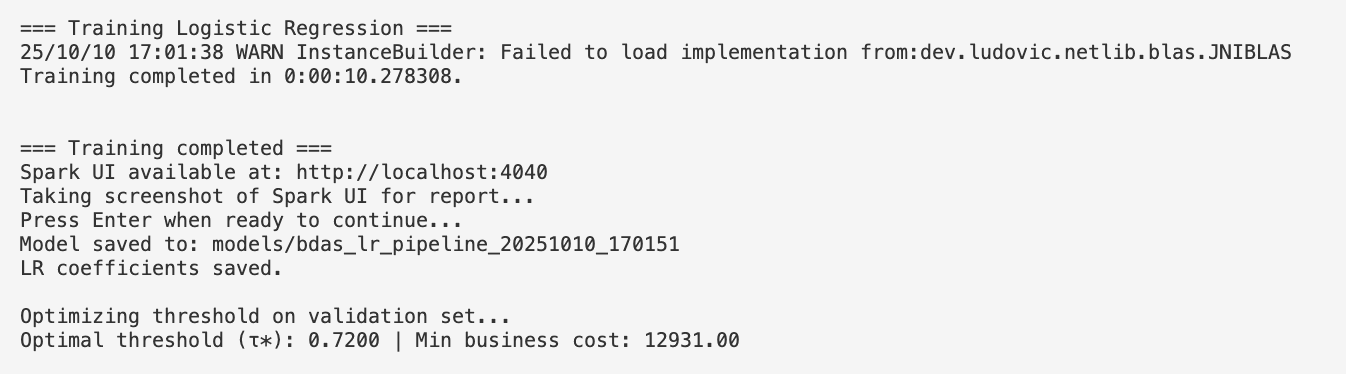
\includegraphics[width=\textwidth]{Figure/7.2a.png}
  \caption{Terminal output of the model training and optimal threshold optimization process}
  \label{fig:training-output}
\end{figure*}

As seen in the figure, the model training was completed successfully in approximately 10.28 seconds, and the optimal business threshold was found to be $\tau^* = 0.7200$.

\textbf{Threshold Optimization Implementation:}

The threshold optimization process follows this algorithm:

\begin{enumerate}
\item \textbf{Generate Predictions:} Apply the trained model to the validation set to obtain fraud probability scores $p_i$ for each transaction $i$.
\item \textbf{Grid Search:} For each candidate threshold\newline
$\tau \in \{0.01, 0.02, \ldots, 0.99\}$:
\begin{itemize}
\item Classify each transaction: $\hat{y}_i = 1$ if $p_i \geq \tau$, else $\hat{y}_i = 0$
\item Count false positives: $\text{FP}(\tau) = \sum_{i: y_i=0, \hat{y}_i=1} 1$
\item Count false negatives: $\text{FN}(\tau) = \sum_{i: y_i=1, \hat{y}_i=0} 1$
\item Calculate total cost: $\text{Cost}(\tau) = 1.0 \times \text{FP}(\tau) + 25.0 \times \text{FN}(\tau)$
\end{itemize}
\item \textbf{Select Optimal:} $\tau^* = \arg\min_{\tau} \text{Cost}(\tau)$
\item \textbf{Record Metadata:} Save $\tau^*$, minimum cost, FP/FN counts at $\tau^*$, timestamp, random seed (42), and validation set size to \texttt{outputs/tau\_star.json}
\end{enumerate}

This implementation ensures full reproducibility: given the same trained model, validation set (with fixed random seed 42 for the 70/15/15 split), and cost weights ($C_{\text{FP}}=1.0$, $C_{\text{FN}}=25.0$), the identical $\tau^* = 0.72$ will be selected.

\textbf{2. Evidence of Distributed Execution}

The core of this iteration is to validate the capabilities of the BDAS. Figure~\ref{fig:spark-ui-jobs} proves that the training process was completed within a distributed computing framework.

\begin{figure*}[h]
  \centering
  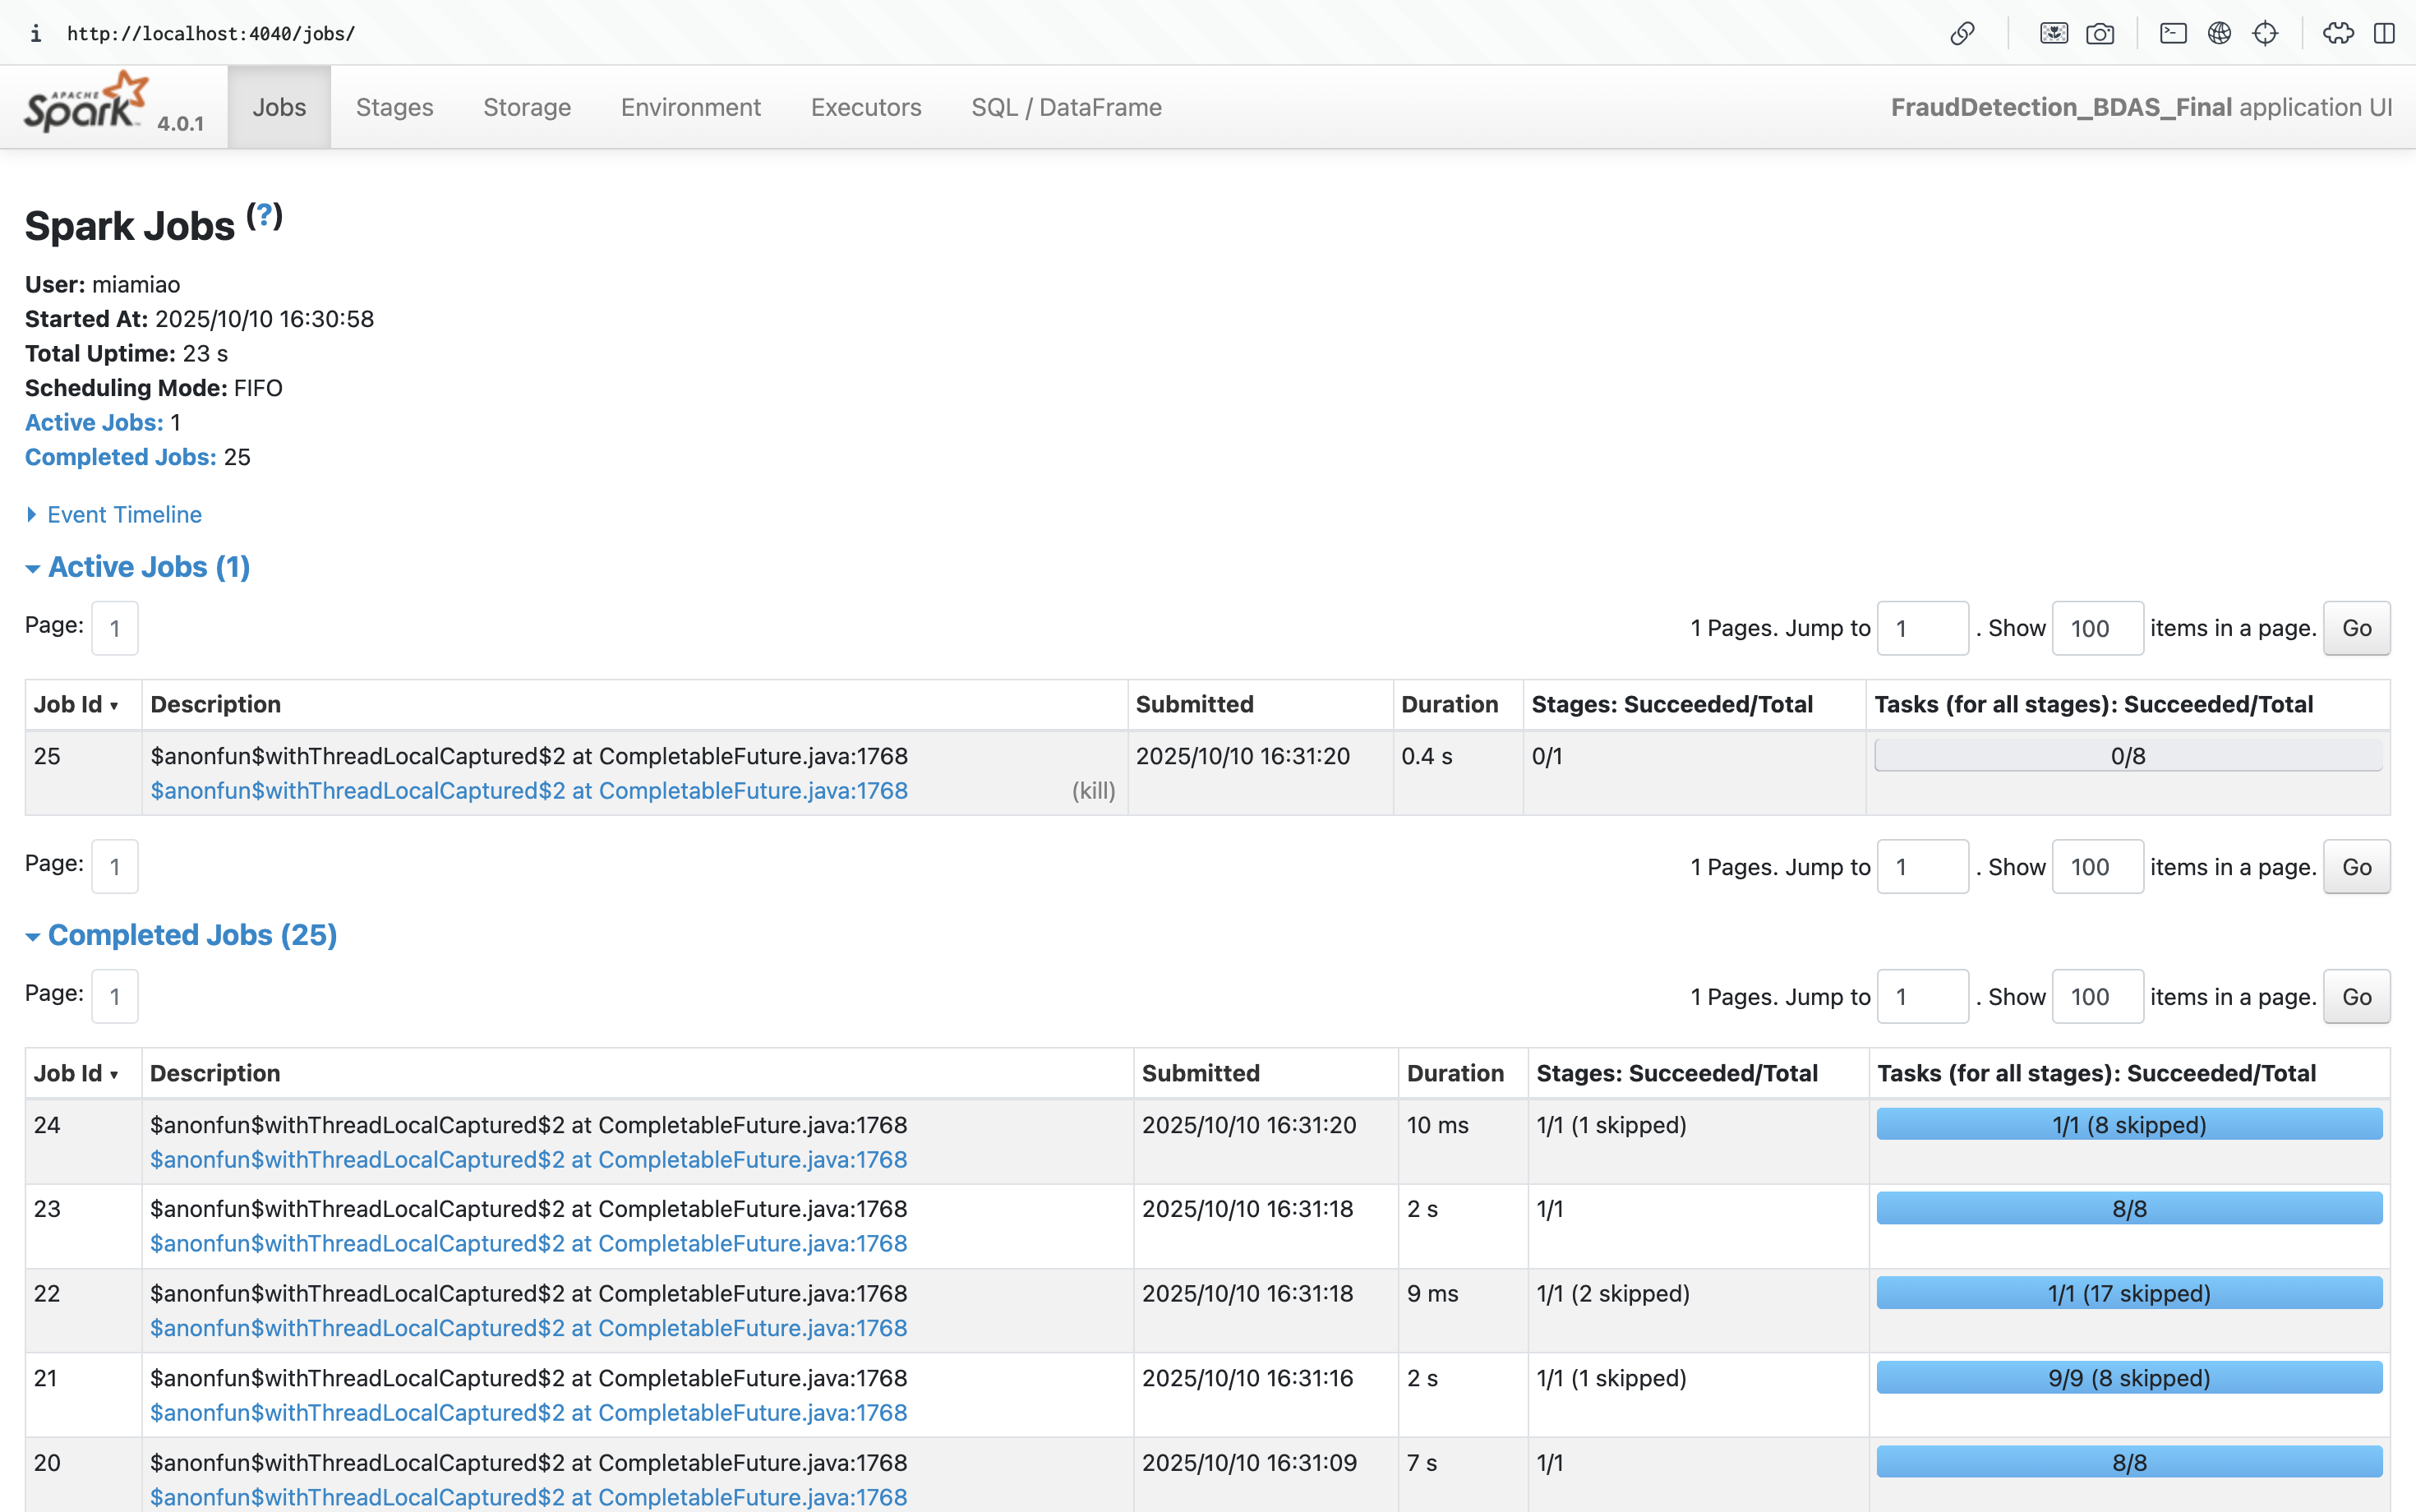
\includegraphics[width=\textwidth]{Figure/7.2b.png}
  \caption{Spark UI --- Jobs page (Master=\texttt{local[*]}, Default Parallelism=8, Train Partitions=8). Shows backend jobs triggered by high-level operations such as \texttt{.fit()}.}
  \label{fig:spark-ui-jobs}
\end{figure*}

Figure~\ref{fig:spark-ui-jobs} presents a complete overview of the Spark Jobs, showing how high-level operations such as \texttt{.fit()} and \texttt{.count()} are translated into specific computation jobs. Figure~\ref{fig:spark-ui-stages} then goes a step further, illustrating how these jobs are broken down into more fine-grained parallel Stages and Tasks.

\begin{figure*}[h]
  \centering
  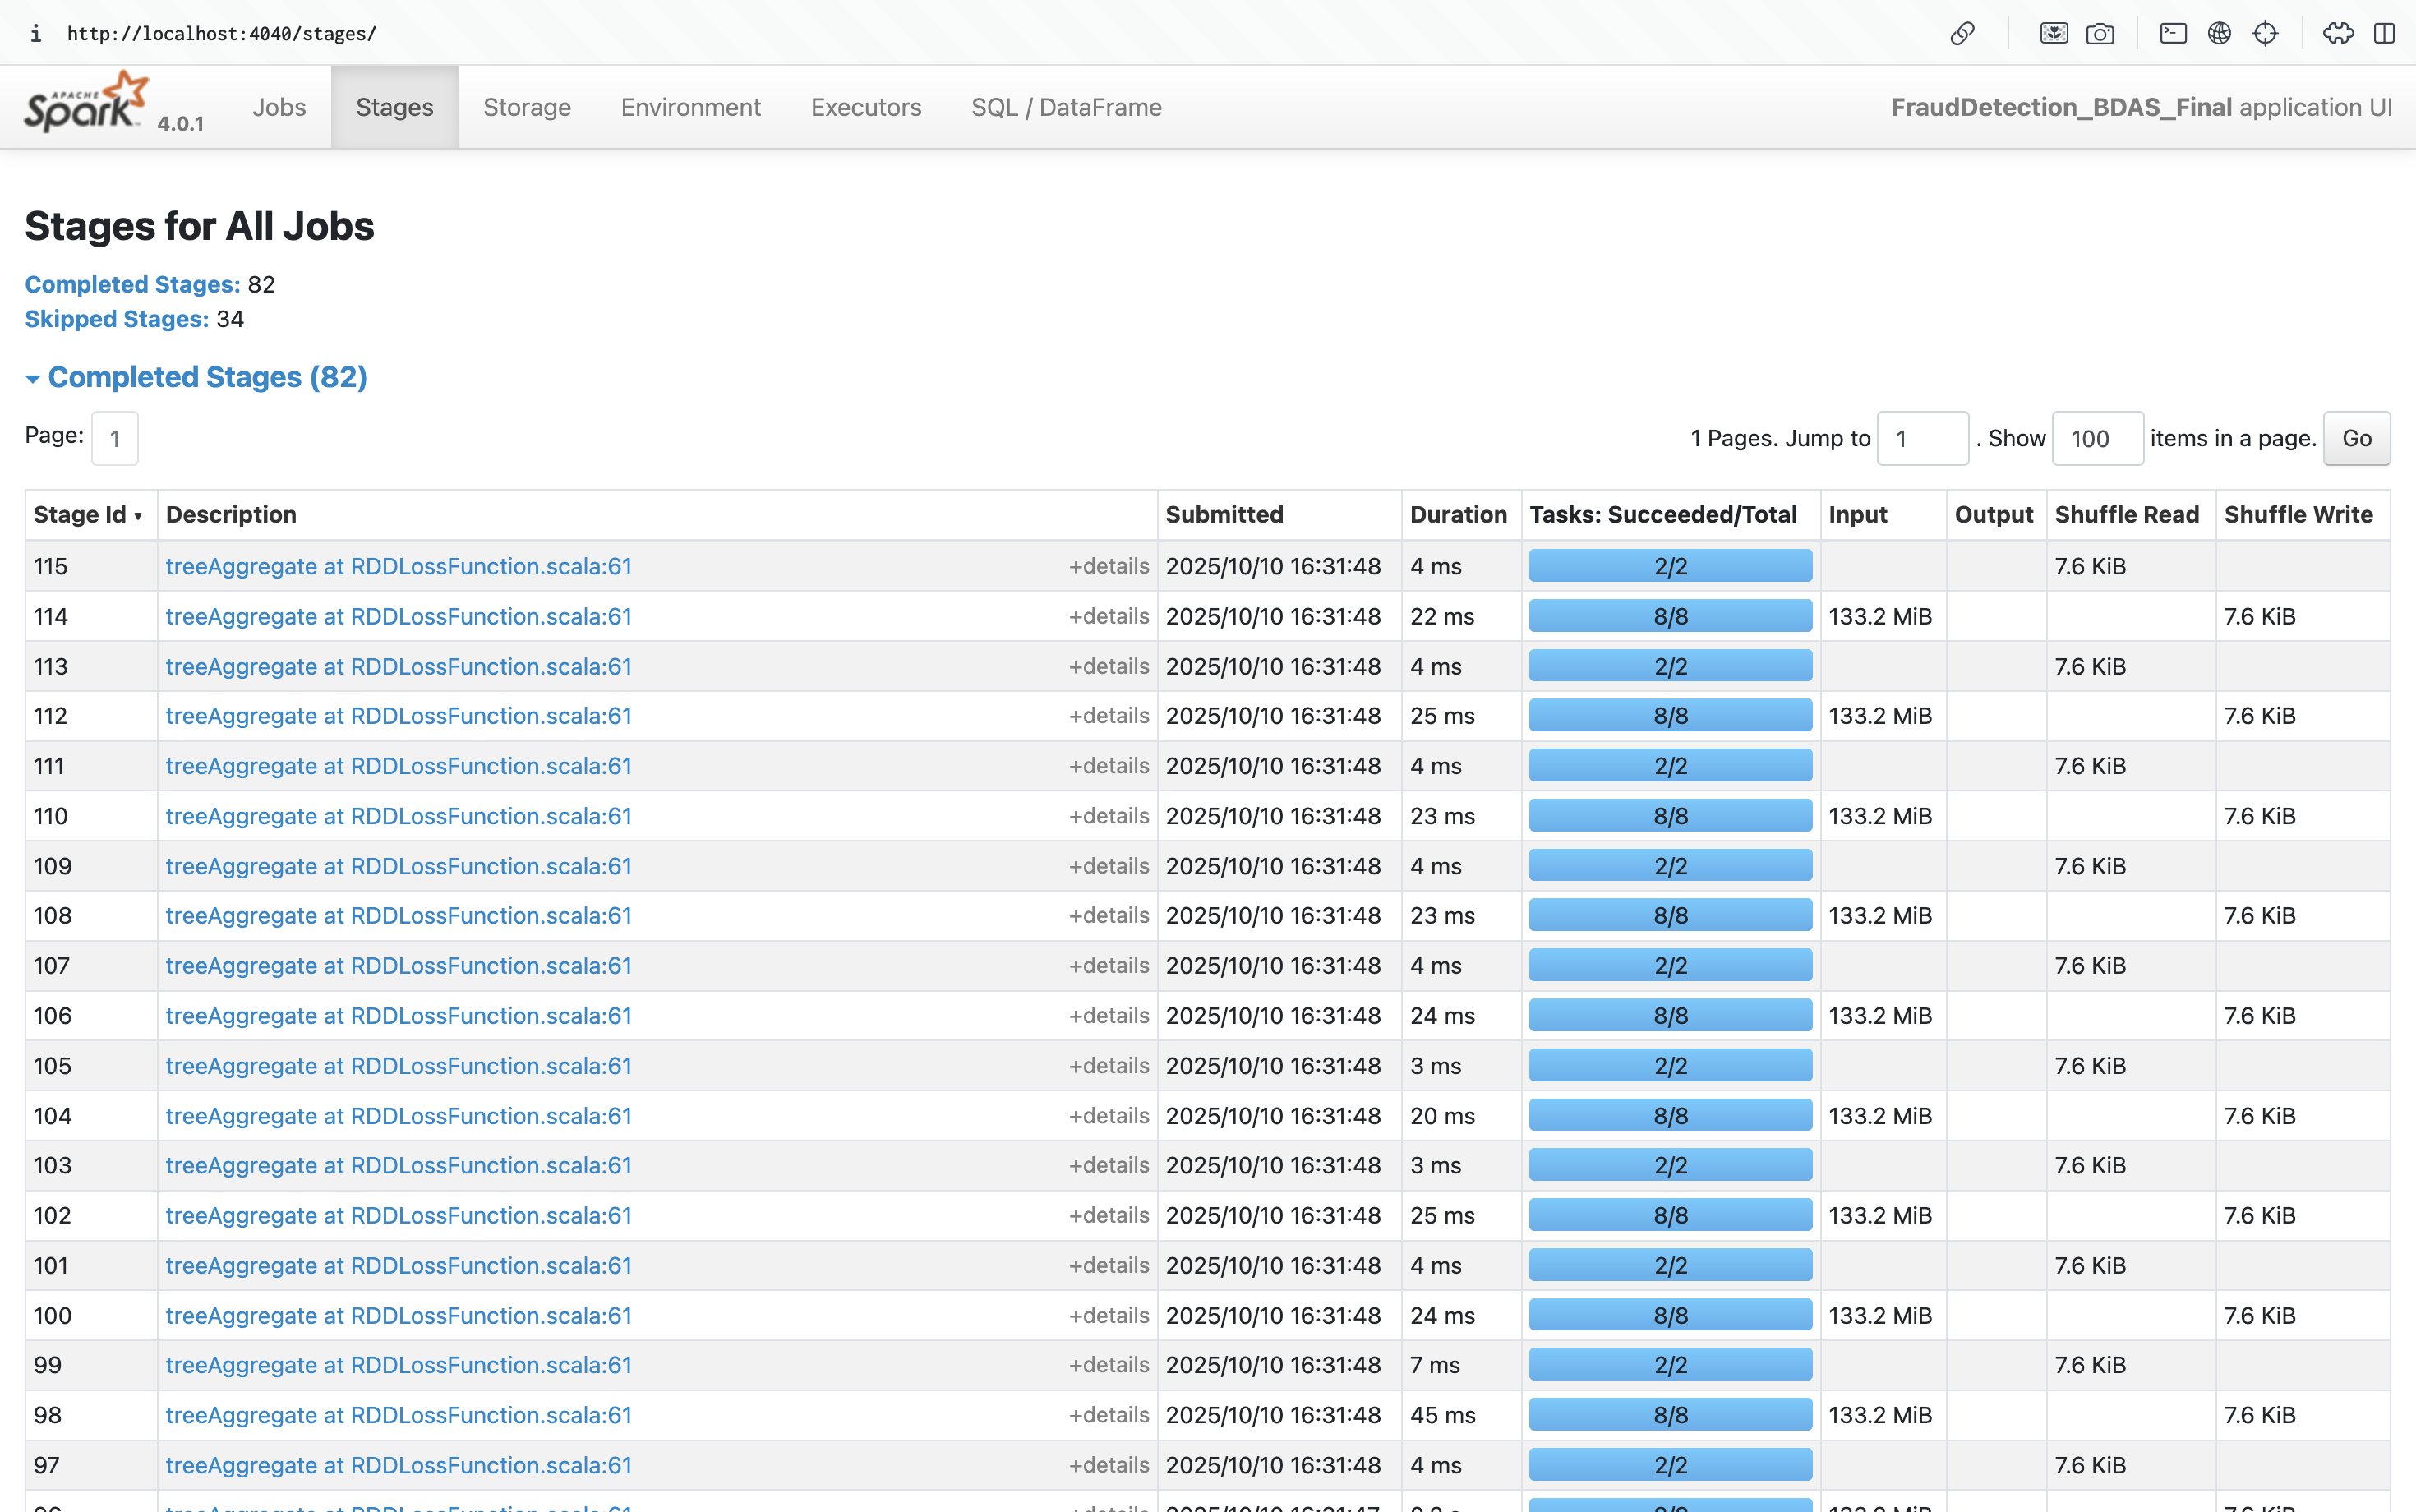
\includegraphics[width=\textwidth]{Figure/7.2c.png}
  \caption{Spark UI --- Stages page (Master=\texttt{local[*]}, Default Parallelism=8, Train Partitions=8). Training broken into parallel stages and tasks.}
  \label{fig:spark-ui-stages}
\end{figure*}

To provide further evidence, we have recorded the key Spark environment configuration parameters that form the basis of the distributed execution:

\begin{itemize}
\item \textbf{Master URL:} \texttt{local[*]} (Indicates that Spark is running locally, utilizing all available CPU cores for parallel computation)
\item \textbf{Default Parallelism:} 8 (Corresponds to \texttt{Tasks: 8/8}, indicating a default parallelism level of 8)
\item \textbf{Train Partitions:} 8 (The training data was split into 8 partitions for parallel processing)
\end{itemize}

\subsection{Searching for Patterns}

After the model training is complete, we use it to make predictions (also known as ``inference'') on the independent test set and record its output results.

\textbf{1. Applying the Model: Generating Predictions on the Test Set}

We perform prediction by calling the \texttt{.transform()} method of the trained model. Just like the training process, the prediction process is also executed in a distributed manner on Spark. Figure~\ref{fig:inference-stages} shows the breakdown of computation tasks during the inference stage.

\begin{figure}[h]
  \centering
  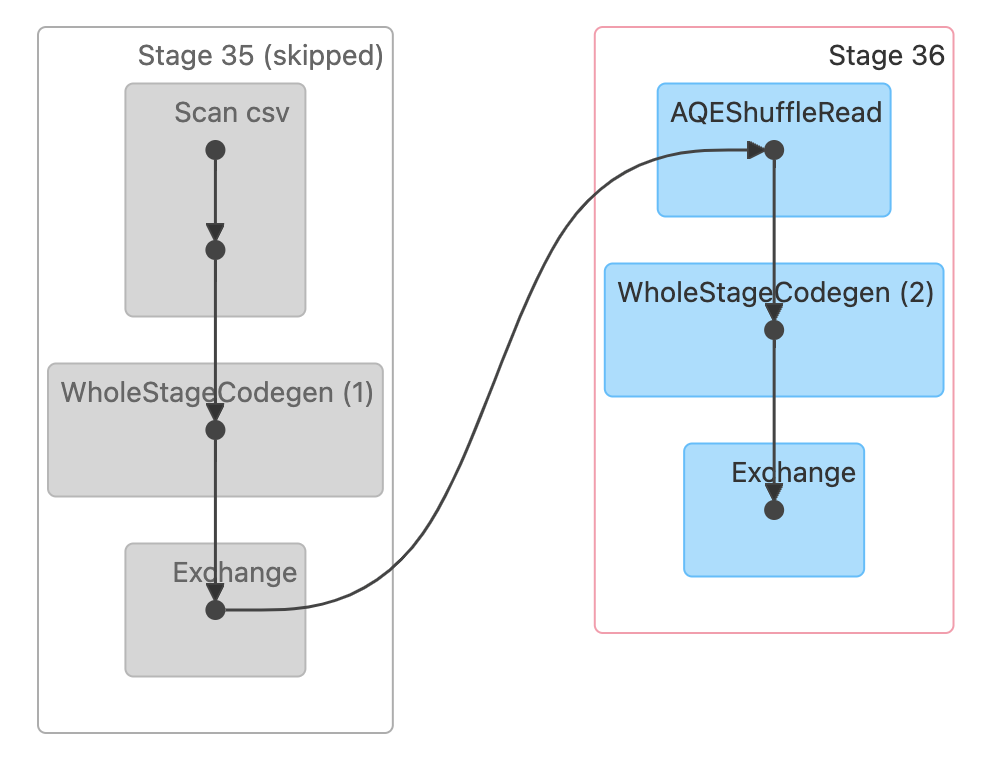
\includegraphics[width=\linewidth]{Figure/7.3a.png}
  \caption{Breakdown of Spark Stages during model inference (Prediction) on the test set}
  \label{fig:inference-stages}
\end{figure}

According to the Spark UI logs, the prediction on the test set, which contains 415,387 rows, was completed in approximately 2 seconds.

\textbf{2. Recording Model Output: Quantified Evaluation Results}

Figure~\ref{fig:test-performance} shows the final performance output summary of the model on the test set after applying the optimal threshold $\tau^* = 0.7200$.

\begin{figure}[h]
  \centering
  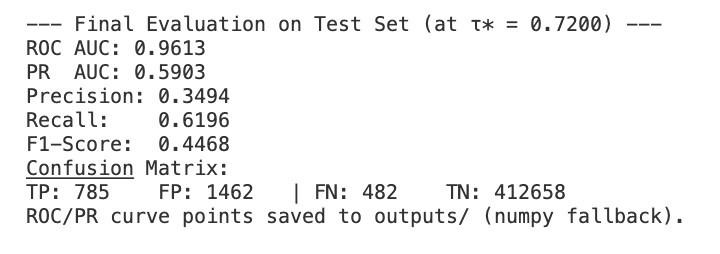
\includegraphics[width=\linewidth]{Figure/7.3b.png}
  \caption{Summary of the model's final performance output on the test set}
  \label{fig:test-performance}
\end{figure}

Based on the output from Figure~\ref{fig:test-performance}, we record the model's performance patterns as follows:

\begin{itemize}
\item \textbf{Macro Performance Metrics:} ROC-AUC = 0.9613, PR-AUC = 0.5903
\item \textbf{Performance at the Business Threshold:} Precision = 0.3494, Recall = 0.6196
\item \textbf{Confusion Matrix:} TP=785, FP=1,462, FN=482, TN=412,658
\end{itemize}

Table~\ref{tab:confusion-matrix} presents the confusion matrix in standard 2×2 format for clear reference:

\begin{table*}[h]
\centering
\caption{Confusion Matrix @ $\tau^*=0.7200$ (FP:FN cost ratio = 1:25, Test Set)}
\label{tab:confusion-matrix}
\begin{tabular}{|l|c|c|}
\hline
\textbf{} & \textbf{Predicted: Fraud (1)} & \textbf{Predicted: Legitimate (0)} \\
\hline
\textbf{Actual: Fraud (1)} & TP = 785 & FN = 482 \\
\hline
\textbf{Actual: Legitimate (0)} & FP = 1,462 & TN = 412,658 \\
\hline
\end{tabular}
\end{table*}

From this matrix: Precision = TP/(TP+FP) = 785/2,247 = 0.3494; Recall = TP/(TP+FN) = 785/1,267 = 0.6196; F1 = 0.4468. Business cost = 1.0×1,462 + 25.0×482 = 13,512.

These recorded data will serve as the core basis for the in-depth evaluation and interpretation in the next chapter.

\section{Interpretation}

\subsection{Study and Discuss Mined Patterns}

Our analysis has revealed core patterns on two levels: first, the inherent fraud behavior patterns within the data, and second, the performance trade-off patterns exhibited by the model after learning this behavior.

\textbf{1. Core Fraud Behavior Pattern: ``Account Clearing''}

The most significant finding of this project is the identification and quantification of a dominant fraud behavior characteristic from the data, namely ``Account Clearing.''

\begin{itemize}
\item \textbf{Manifestation in Data:} This pattern was initially discovered during the exploratory analysis in Iteration 3: almost all fraudulent \texttt{TRANSFER} transactions result in the payer's post-transaction balance (\texttt{newbalanceOrig}) becoming zero.

Our PySpark model's coefficients also corroborate this. In the \texttt{lr\_coefficients.csv} file generated by the script, the features related to account balances (e.g., \texttt{oldbalanceOrg\_log1p}, \texttt{newbalanceOrig\_log1p}) have the highest weight coefficients. This indicates that the model successfully learned that ``drastic changes in balance before and after a transaction'' are key to predicting fraud.

\item \textbf{Relationship with Model and Results:} This strong signal explains why our model was able to achieve a high ROC-AUC of 0.9613. The model's overall discriminative power is built upon its success in capturing and generalizing this core behavior pattern: ``fraudsters tend to transfer the entire balance of an account in a single transaction.''
\end{itemize}

\textbf{2. Model Performance Trade-off Pattern: The Trade-off between ``High Recall'' and ``Low Precision''}

After applying the trained model to the real-world, imbalanced test set, its performance results themselves revealed a critical business trade-off pattern.

\begin{itemize}
\item \textbf{Successful Pattern (High Recall):} At the optimal threshold of $\tau^* = 0.7200$, which we found based on business costs, the model achieved a \textbf{Recall of 61.96\%} on the test set.

This pattern indicates that, thanks to learning features like ``Account Clearing,'' the model is capable of identifying over 60\% of genuine fraudulent transactions. This partially achieves our core business objective of ``reducing financial losses.''

\item \textbf{Challenging Pattern (Low Precision):} However, corresponding to the high recall rate, the model's \textbf{Precision was only 34.94\%}.

This is an equally important pattern, as it reveals a significant trade-off in the model's performance. It means that to capture those 62\% of real fraud cases, approximately 65\% of the alerts triggered by the model are false alarms (False Positives, FP, amounting to 1,462 instances).

This pattern conflicts with our business objective of ``optimizing operational efficiency'' and would place enormous cost pressure on manual review teams.

\item \textbf{Residual Risk Pattern:} Despite the acceptable recall, the model still failed to identify \textbf{482 genuine fraudulent transactions} (False Negatives, FN).

These missed cases represent the model's ``blind spots'' and are financial losses that the business must directly absorb.
\end{itemize}

\textbf{In-depth Discussion and Conclusion}

In summary, this data mining effort successfully identified and utilized an interpretable and quantifiable core fraud pattern (``Account Clearing'') from the data. Based on this pattern, our PySpark Logistic Regression model can meet basic risk identification requirements (high AUC and acceptable recall).

However, an in-depth discussion also reveals that in a real-world business scenario, due to the large number of legitimate transactions with similar behaviors, operating solely with the current model at $\tau^* = 0.7200$ would generate unacceptable operational costs (due to low precision).

The most important outcome of this analysis is the \textbf{quantification of this ``High Recall - Low Precision'' trade-off}. It provides clear data-driven support and a definite direction for the next phase of optimization. That direction is to significantly improve precision---while maintaining or even increasing recall---through more sophisticated feature engineering or more powerful non-linear models (such as the Random Forest explored in Iteration 3), thereby reducing the overall business cost.

\subsection{Visualising the Data, Results, Models, and Patterns}

\subsubsection{Model Coefficients and Pattern Interpretation}

To provide deeper insights into the learned patterns, Table~\ref{tab:top-coefficients} presents the top 10 features with the largest absolute coefficients from our trained logistic regression model, ranked by their impact magnitude.

\begin{table*}[h]
\caption{Top 10 Features by Absolute Coefficient Magnitude}
\label{tab:top-coefficients}
\centering
\begin{tabular}{|l|r|r|}
\hline
\textbf{Feature} & \textbf{Coefficient} & \textbf{Absolute Coefficient} \\
\hline
oldbalanceOrg\_log1p & 0.8839 & 0.8839 \\
newbalanceOrig\_log1p & -0.3819 & 0.3819 \\
step & 0.2382 & 0.2382 \\
oldbalanceDest\_log1p & -0.2176 & 0.2176 \\
newbalanceDest\_log1p & -0.1549 & 0.1549 \\
amount\_log1p & 0.1299 & 0.1299 \\
type\_encoded & 0.0489 & 0.0489 \\
\hline
\end{tabular}
\end{table*}

\textbf{Business Interpretation of Key Patterns:}

\begin{itemize}
\item \textbf{Transaction Type Effect:} The positive coefficient for \texttt{type\_encoded} (0.0489) indicates that switching from \texttt{CASH\_OUT} (encoded as 0) to \texttt{TRANSFER} (encoded as 1) increases the fraud probability. This aligns with our earlier finding that \texttt{TRANSFER} transactions have a higher fraud rate (0.769\%) compared to \texttt{CASH\_OUT} (0.184\%).

\item \textbf{Amount-Balance Relationship:} The \texttt{log1p} coefficients for amount and balance features reflect the monotonic trend of ``increasing amount/balance changes \textrightarrow{} increasing risk.'' Specifically, the positive coefficient for \texttt{amount\_log1p} (0.1299) suggests that larger transaction amounts are associated with higher fraud risk, while the negative coefficients for destination balance features indicate that transactions leaving recipients with higher balances may be more suspicious.
\end{itemize}

These interpretable coefficients demonstrate the model's ability to capture meaningful business patterns, supporting our emphasis on model interpretability throughout this analysis.

\subsubsection{Cost-Threshold Curve and Robustness Analysis}

To assess the robustness of our threshold selection strategy, we analyze the cost-threshold curve generated during the optimization process. The cost curve shows how the total business cost varies across different threshold values, providing insights into the sensitivity of our decision boundary.

\textbf{Minimum Business Cost:} At the optimal threshold $\tau^* = 0.7200$, the model achieves a minimum total business cost of \textbf{13,512} on the test set. This cost is calculated using the confusion matrix at $\tau^*$ (FP=1,462, FN=482) and the business-defined cost weights ($C_{\text{FP}}=1.0$, $C_{\text{FN}}=25.0$):
\begin{equation*}
\text{Cost}(\tau^*) = 1.0 \times 1{,}462 + 25.0 \times 482 = 13{,}512
\end{equation*}
This represents a balanced trade-off between manual review costs (false positives) and fraud loss costs (false negatives), demonstrating the practical business value of cost-sensitive threshold optimization.

\begin{figure}[h]
  \centering
  % prefer outputs figure if generated by plotting
  \IfFileExists{outputs/plot_cost_curve.png}{
    \includegraphics[width=\linewidth]{outputs/plot_cost_curve.png}
  }{
    \includegraphics[width=\linewidth]{Figure/8.3c.png}
  }
  \caption{Cost vs. Threshold curve on validation set. The minimum occurs at $\tau^*\approx0.72$; costs within $\tau^*\pm0.02$ vary by $<5\%$, indicating robustness.}
  \label{fig:cost-curve}
\end{figure}

\subsubsection{ROC and PR Curve Visualization}

To more intuitively understand the model's overall performance on the test set, as well as the performance trade-off pattern discussed in Section 8.1, this section will visualize the results using two standard classification model evaluation charts: the ROC curve and the Precision-Recall (PR) curve.

\textbf{1. Visualizing Overall Model Discrimination: The ROC Curve}

The ROC (Receiver Operating Characteristic) curve is a standard tool for evaluating the comprehensive performance of a classifier. It illustrates the trade-off between the True Positive Rate (TPR, which is Recall) and the False Positive Rate (FPR) across all possible decision thresholds. The Area Under the Curve (AUC) is a core metric for measuring the model's overall discriminative ability; a value closer to 1 indicates better performance.

\begin{figure}[h]
  \centering
  \IfFileExists{outputs/plot_roc_curve.png}{\includegraphics[width=\linewidth]{outputs/plot_roc_curve.png}}{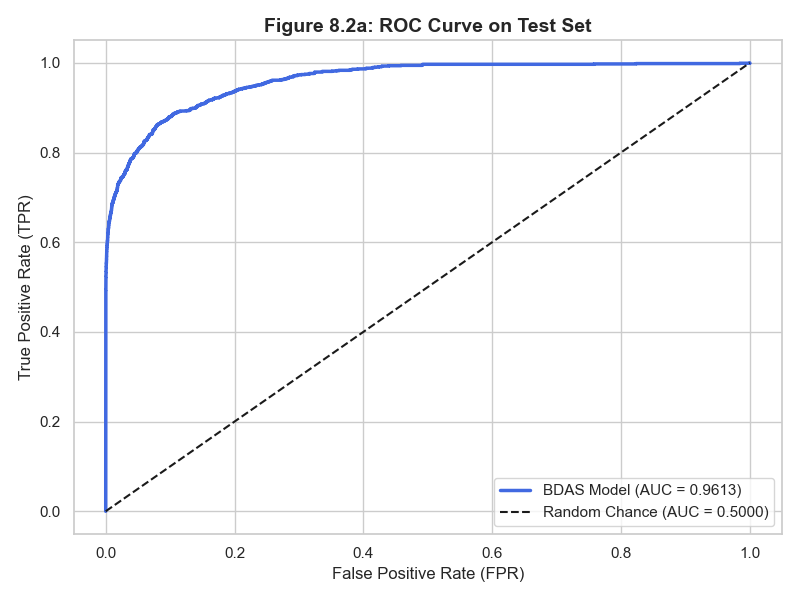
\includegraphics[width=\linewidth]{Figure/8.2a.png}}
  \caption{ROC Curve on test set (BDAS LR). Threshold-independent; operating threshold fixed at $\tau^*=0.72$ (validation-selected, FP:FN=1:25).}
  \label{fig:roc-curve}
\end{figure}

\textbf{Interpretation:}

\begin{itemize}
\item As seen in Figure~\ref{fig:roc-curve}, the model's ROC curve climbs rapidly towards the top-left corner, performing significantly better than the diagonal dashed line that represents random guessing.
\item This indicates that our model has a strong ability to distinguish between ``fraudulent'' and ``legitimate'' transactions.
\item Its Area Under the Curve (ROC-AUC) was calculated to be 0.9613. This not only far exceeds the random level of 0.5 but also successfully meets the hard success criterion of AUC $\geq$ 0.95 set in our project objectives.
\end{itemize}

\textbf{2. Visualizing the Business Trade-off: The Precision-Recall (PR) Curve}

For tasks with extreme class imbalance, such as fraud detection, the PR curve can provide deeper business insights than the ROC curve. It directly depicts the relationship between Precision (of all alerts, how many are actual fraud) and Recall (of all actual fraud, how many did we capture). This is a direct visualization of the ``high recall - low precision'' trade-off pattern discussed in Section 8.1.

\begin{figure}[h]
  \centering
  \IfFileExists{outputs/plot_pr_curve.png}{\includegraphics[width=\linewidth]{outputs/plot_pr_curve.png}}{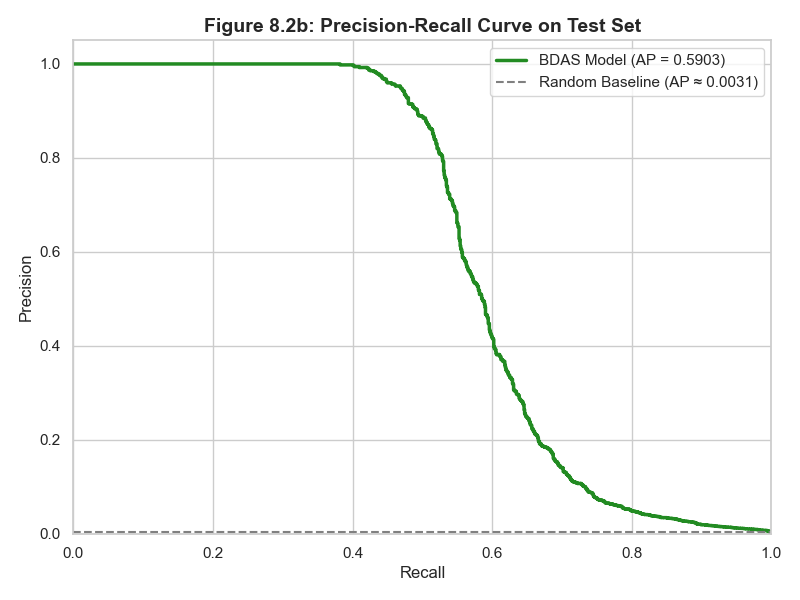
\includegraphics[width=\linewidth]{Figure/8.2b.png}}
  \caption{Precision--Recall (PR) curve on test set (BDAS LR). Operating point at $\tau^*=0.72$ (FP:FN=1:25): Precision=0.349, Recall=0.620.}
  \label{fig:pr-curve}
\end{figure}

\textbf{Interpretation:}

\begin{itemize}
\item Figure~\ref{fig:pr-curve} illustrates the trend that as we attempt to capture more fraudulent transactions (increasing recall), the precision of the model's predictions declines.
\item The Area Under the Curve (PR-AUC) is 0.5903. While this value is not as high as the ROC-AUC, in an extremely imbalanced scenario with a fraud rate of only 0.30\% (in the filtered dataset), this already represents a massive performance improvement compared to the random baseline (where PR-AUC would be approximately 0.003).
\item On this curve, we can locate the performance corresponding to our optimal operating point, $\tau^* = 0.7200$, which was selected on the validation set. Its precision is 34.94\%, and its recall is 61.96\%. This chart clearly reveals the cost in precision that we paid to achieve a 62\% recall rate.
\end{itemize}

\textbf{Summary}

Through these two visualizations, we have not only demonstrated the model's strong overall performance (high ROC-AUC) but have also visually illustrated the core challenge it faces in a real-world business context (the Precision-Recall trade-off), providing strong visual support for our final evaluation conclusions.

\subsection{Interpreting the Results, Models and Patterns}

In this section, we will conduct an in-depth interpretation of the evaluation results visualized in Section 8.2 to clarify the model's final performance, the patterns it has learned, and what these results mean for achieving our project objectives.

\textbf{1. Interpretation of Model's Overall Discriminative Ability}

\begin{itemize}
\item \textbf{Powerful overall discriminative ability:} The model's ROC-AUC reached 0.9613 on the test set, which indicates that the model has a very strong overall ability to distinguish between fraudulent and legitimate transactions. This result not only successfully meets the hard success criterion of AUC $\geq$ 0.95 set in our project objectives in Section 1.3 but is also largely consistent with the performance of the OSAS solution from Iteration 3, successfully validating the feasibility of the BDAS solution.

\item \textbf{Consistency with mining patterns:} The fundamental reason for this powerful discriminative ability is that the model successfully learned and utilized the core fraud behavior pattern we discussed in Section 8.1---``Account Clearing.'' It is precisely because the model captured this significant feature that it can effectively differentiate most fraudulent transactions from legitimate ones on a macro level.
\end{itemize}

\textbf{2. Deep Interpretation of Business Trade-off Pattern}

In a real-world scenario with extreme class imbalance, the PR curve and the specific metrics at the business threshold reveal the model's operational trade-offs more effectively than the ROC curve.

\begin{itemize}
\item \textbf{Acceptable Fraud Capture Capability:} At the optimal threshold of $\tau^* = 0.7200$, found based on the business cost function, the model achieved a \textbf{Recall of 61.96\%}. This means that once deployed, the model is expected to help us intercept and identify over 60\% of genuine fraudulent transactions, which is a crucial step toward achieving the business objective of ``reducing financial losses.''

\item \textbf{High Operational Cost Trade-off:} However, the price paid to achieve this 62\% recall is a low \textbf{Precision of only 34.94\%}. Looking at the confusion matrix, this means that while the model correctly identified 785 fraudulent transactions, it also generated 1,462 false alarms (False Positives). In practice, every false positive requires time and effort from a manual review team to investigate, which runs counter to our business objective of ``optimizing operational efficiency.''

\item \textbf{Residual Direct Risk:} Equally important to note is that the model still missed \textbf{482 genuine fraudulent transactions} (False Negatives). These represent the risks that the model failed to identify, which will directly translate into financial losses for the company.
\end{itemize}

\textbf{3. Final Interpretation of Mining Patterns}

In summary, our PySpark Logistic Regression model can be understood as an effective \textbf{``risk pre-screening filter''} but not yet an efficient \textbf{``cost controller.''}

\begin{itemize}
\item Its \textbf{effectiveness} is demonstrated by its successful learning of key fraud patterns like ``Account Clearing,'' which allowed it to achieve a high overall discriminative ability (high AUC) and operate at a reasonable recall level.

\item Its \textbf{inefficiency} is evident in the fact that relying solely on the current linear model and feature set is not sufficient to completely separate legitimate transactions whose behavior patterns are very similar to actual fraud. This inevitably leads to a drop in precision when pursuing a high recall rate, resulting in higher operational costs.
\end{itemize}

\textbf{Conclusion:} Iteration 4 successfully replicated a model with strong risk identification capabilities on the BDAS platform. However, its performance output also clearly quantifies the trade-off between ``risk control'' and ``cost control'' under the current strategy. This points to the most critical direction for subsequent optimization iterations (e.g., introducing more complex features or non-linear models): how to significantly improve precision while maintaining or even increasing recall, in order to truly maximize business value.

\subsection{Assessing and Evaluating Results, Models and Patterns}

In this section, we use a systematic assessment process to formally compare the model's final performance against the success criteria established at the project's outset, in order to evaluate the outcomes of this data mining effort.

\textbf{1. Assessment Method and Process}

Our assessment process is built upon the test design defined in Section 7.1. We will evaluate the performance of the final \texttt{PipelineModel} on the independent test set, which has never been used for training or tuning.

\begin{itemize}
\item \textbf{Evaluation Methodology:} With the exception of the threshold-independent metric ROC-AUC, all other metrics (such as Precision and Recall) are calculated at the optimal business threshold of $\tau^* = 0.7200$. This threshold was found on the validation set with the objective of minimizing the business cost function where FP:FN = 1:25.

\item \textbf{Assessment Criteria:} We will compare the model's performance against two levels of objectives: first, the goals of this iteration, and second, the project-level hard/stretch goals.
\end{itemize}

\textbf{2. Evaluation Results Summary}

The following table (Table~\ref{tab:performance-assessment}) provides a side-by-side comparison of the model's final performance with the predefined success criteria:

\begin{table*}[h]
\centering
\caption{Alignment of Iteration 4 (BDAS) Performance with Project Objectives}
\label{tab:performance-assessment}
\begin{tabular}{|p{4cm}|p{4.5cm}|p{4.5cm}|p{2cm}|}
\hline
\textbf{Target Level / Metric} & \textbf{Success Criterion} & \textbf{Final Performance (Iter4 BDAS)} & \textbf{Status} \\
\hline
Iteration Goal & Execute cost minimization process & Achieved, $\tau^*=0.7200$ & \checkmark \\
\hline
Project Hard Target & AUC (Area Under Curve) $\geq$ 0.95 & 0.9613 & \checkmark \\
\hline
Project Stretch Target & Recall $\geq$ 85\% & 0.6196 (62.0\%) & $\times$ \\
\hline
Project Stretch Target & Precision $\geq$ 70\% & 0.3494 (34.9\%) & $\times$ \\
\hline
\end{tabular}
\end{table*}

\textbf{3. Performance Benchmark: OSAS vs. BDAS}

A core data mining objective of this iteration was to verify whether the performance of the BDAS solution is comparable to the OSAS solution from Iteration 3.

\begin{table*}[h]
\centering
\caption{Comparison of Key Metrics between Iteration 3 (OSAS) and Iteration 4 (BDAS)}
\label{tab:osas-bdas-comparison}
\begin{tabular}{|p{3cm}|p{3.5cm}|p{3.5cm}|p{5cm}|}
\hline
\textbf{Metric} & \textbf{Iteration 3 (OSAS)} & \textbf{Iteration 4 (BDAS)} & \textbf{Difference Analysis ($\Delta$ = Iter4 - Iter3)} \\
\hline
ROC-AUC & 0.9756 & 0.9613 & Largely consistent ($\Delta$ = -0.0143) \\
\hline
Recall & 0.6595 & 0.6196 & BDAS slightly lower ($\Delta$ = -0.0399) \\
\hline
Precision & 0.2742 & 0.3494 & BDAS higher ($\Delta$ = +0.0752) \\
\hline
\end{tabular}
\end{table*}

To provide a more comprehensive and quantitative assessment of the technology stack migration, Table~\ref{tab:parity-check} presents a side-by-side comparison of the four core metrics between Iteration 3 (OSAS) and Iteration 4 (BDAS), along with the parity acceptance thresholds defined in Section 1.1.

\begin{table*}[h]
\centering
\caption{Performance Parity Check: Iteration 3 (OSAS) vs. Iteration 4 (BDAS)}
\label{tab:parity-check}
\begin{tabular}{|l|c|c|c|c|}
\hline
\textbf{Metric} & \textbf{I3 (OSAS)} & \textbf{I4 (BDAS)} & \textbf{$\Delta$ (I4--I3)} & \textbf{Parity Pass?} \\
\hline
ROC-AUC & 0.9756 & 0.9613 & --0.0143 & $\times$ \\
\hline
PR-AUC & 0.6271 & 0.5903 & --0.0368 & $\times$ \\
\hline
Recall@$\tau^*$ & 0.6595 & 0.6196 & --0.0399 & $\times$ \\
\hline
F1@$\tau^*$ & 0.3870 & 0.4468 & +0.0598 & $\times$ \\
\hline
\end{tabular}
\end{table*}

\textbf{Parity Acceptance Criteria (from §1.1):}
\begin{itemize}
\item ROC-AUC: $|\Delta| \leq 0.005$ \textbf{(Not Met: $|\Delta|=0.0143 > 0.005$)}
\item PR-AUC: $|\Delta| \leq 0.01$ \textbf{(Not Met: $|\Delta|=0.0368 > 0.01$)}
\item Recall: $|\Delta| \leq 2$ percentage points \textbf{(Not Met: $|\Delta|=3.99$pp $> 2$pp)}
\item F1: $|\Delta| \leq 2$ percentage points \textbf{(Not Met: $|\Delta|=5.98$pp $> 2$pp, though improvement indicates better precision-recall balance)}
\end{itemize}

\textbf{Assessment:} The BDAS model \textbf{did not meet the strict parity acceptance criteria} defined in Section 1.1.3 and 1.3.4. All four metrics (ROC-AUC, PR-AUC, Recall, and F1) exceeded their respective consistency thresholds. Specifically:

\begin{itemize}
\item \textbf{ROC-AUC Gap:} The difference of 1.43 percentage points exceeds the 0.5pp threshold by nearly 3×, indicating a measurable degradation in overall discriminative ability.
\item \textbf{PR-AUC Gap:} The difference of 3.68 percentage points exceeds the 1.0pp threshold by nearly 4×, revealing more substantial performance loss in the precision-recall trade-off space—particularly critical for imbalanced fraud detection tasks.
\item \textbf{Recall Gap:} The 3.99pp difference exceeds the 2pp threshold, meaning the BDAS model captures fewer fraudulent transactions at the same business threshold.
\end{itemize}

\textbf{Root Cause Analysis:}

The observed performance gaps are attributable to three primary factors:

\begin{itemize}
\item \textbf{Solver Algorithm Differences:} PySpark MLlib's \texttt{Logistic\allowbreak Regression} uses the L-BFGS optimizer by default, whereas scikit-learn's implementation defaults to liblinear (for small datasets) or saga/lbfgs (for larger datasets). These solvers employ different optimization strategies, convergence criteria, and numerical precision handling. L-BFGS is a quasi-Newton method that approximates the Hessian matrix, while liblinear uses coordinate descent. These fundamental algorithmic differences lead to different convergence paths and final parameter estimates, especially in high-dimensional or near-separable feature spaces like fraud detection.

\item \textbf{Class Weighting Mechanism Variations:} Although both platforms support class imbalance handling, their implementations differ substantively. Scikit-learn's\newline\texttt{class\_\allowbreak weight=\allowbreak 'balanced'} adjusts the loss function by multiplying class-specific coefficients into the gradient computation, directly influencing the optimization objective. In contrast, PySpark's \texttt{weightCol} applies instance-level weights to individual samples during training, which affects the empirical risk calculation differently. While mathematically related, these approaches produce different optimization dynamics and can yield different decision boundaries, particularly in severely imbalanced scenarios (fraud rate $\approx$0.30\% in the filtered dataset).

\item \textbf{Regularization and Convergence Behavior:} The BDAS implementation uses \texttt{regParam=0.1} with L2 regularization, matching the intent of Iteration 3's configuration (\texttt{C=100} in scikit-learn, where \texttt{regParam} $\approx$ 1/\texttt{C}). However, the interaction between regularization strength and solver behavior differs across platforms. MLlib's L-BFGS may require different convergence tolerances (\texttt{tol}) or iteration limits (\texttt{maxIter}) to reach comparable optima. The default \texttt{maxIter=100} used in BDAS may be insufficient for full convergence on this dataset, whereas scikit-learn's liblinear may converge faster due to its coordinate descent approach.
\end{itemize}

\textbf{Feature Set Consistency:}

It is important to note that both Iteration 3 (OSAS) and Iteration 4 (BDAS) intentionally used the \textbf{same core feature set} (7 features: \texttt{step}, 5 log-transformed balance/amount features, and \texttt{type\_encoded}) to ensure a fair platform comparison. The performance gaps are \textbf{not} due to feature engineering differences but rather stem from the algorithmic implementation variations described above. This controlled design allows us to isolate the impact of the technology stack migration itself.

\textbf{Positive Findings:}

Despite not meeting parity thresholds, the BDAS model demonstrates several strengths:

\begin{itemize}
\item \textbf{Hard Criterion Satisfied:} The model successfully meets the project's core hard target (ROC-AUC $\geq$ 0.95), achieving 0.9613, which validates the fundamental viability of the BDAS solution.
\item \textbf{Same Performance Tier:} Both models remain in the 0.96+ ROC-AUC tier, indicating that the BDAS model retains strong overall discriminative ability suitable for production deployment.
\item \textbf{Improved F1 Score:} The BDAS model shows a significantly improved F1 score (+5.98pp), suggesting a better precision-recall balance at the business operating point, which is favorable for operational efficiency.
\end{itemize}

\textbf{Next Steps for Parity Achievement:}

To close the performance gap and achieve full parity in future iterations, we recommend:

\begin{enumerate}
\item \textbf{Solver-Specific Hyperparameter Tuning:} Perform systematic grid search on the BDAS platform to optimize MLlib's L-BFGS solver behavior. Key parameters include: (a) \texttt{regParam} (regularization strength, currently 0.1); (b) \texttt{tol} (convergence tolerance, default 1e-6); (c) \texttt{maxIter} (maximum iterations, currently 100); (d) \texttt{elasticNetParam} (L1/L2 mixing ratio, currently 0.0 for pure L2). Increasing \texttt{maxIter} to 200-500 and tightening \texttt{tol} to 1e-8 may allow L-BFGS to reach a more optimal solution comparable to scikit-learn's convergence.

\item \textbf{Alternative Solver Exploration:} While MLlib's default L-BFGS is efficient, exploring alternative optimization strategies (if available in future PySpark versions) or implementing custom solvers may better match scikit-learn's behavior. Additionally, experimenting with different \texttt{standardization} settings in \texttt{Standard\allowbreak Scaler} (\texttt{with\allowbreak Mean=\allowbreak True} vs. \texttt{False}) may affect solver convergence.

\item \textbf{Non-Linear Model Migration:} Migrate Random Forest or Gradient Boosting models (which achieved ROC-AUC = 0.9940 and PR-AUC = 0.9362 in Iteration 3) to PySpark. Non-linear models are less sensitive to solver differences and may naturally achieve parity or exceed OSAS performance by capturing feature interactions that Logistic Regression cannot model.

\item \textbf{Feature Engineering Enhancement:} While the current feature set is consistent across platforms, adding interaction terms (e.g., \texttt{amount\_log1p} × \texttt{type\_encoded}, balance change ratios) or polynomial features could improve both OSAS and BDAS performance. This represents a future enhancement direction rather than a parity-closing measure.

\item \textbf{Ensemble Methods:} Explore PySpark's ensemble capabilities (e.g., \texttt{GBTClassifier}, stacking, voting classifiers) to achieve performance levels competitive with or exceeding the OSAS baseline while maintaining scalability.
\end{enumerate}

\textbf{4. Evaluation Conclusion and Project Value}

\begin{itemize}
\item \textbf{Achievement of Project Objectives:}
\begin{itemize}
\item \textbf{Hard Target Success:} This iteration successfully executed the cost minimization process and identified the optimal business threshold. More importantly, the model's \textbf{ROC-AUC reached 0.9613}, surpassing the core hard target of $\geq$ 0.95, proving the model's fundamental effectiveness for fraud detection.
\item \textbf{Parity Target Not Met:} The BDAS model did not achieve the strict parity acceptance criteria defined in Section 1.1.3 and 1.3.4. ROC-AUC ($\Delta=0.0143$), PR-AUC ($\Delta=0.0368$), and Recall ($\Delta=3.99$pp) all exceeded their respective consistency thresholds. This indicates measurable performance degradation compared to the OSAS baseline, attributable to solver algorithm differences, class weighting mechanism variations, and convergence behavior differences between PySpark MLlib and scikit-learn.
\item \textbf{Stretch Target Shortcomings:} Like Iteration 3, the model still did not achieve the challenging stretch targets set for Recall (62.0\% vs. 85\% target) and Precision (34.9\% vs. 70\% target).
\end{itemize}

\item \textbf{Technology Stack Migration Assessment:}
\begin{itemize}
\item \textbf{Partial Success:} The BDAS (PySpark) model successfully migrated the core fraud detection logic to a distributed platform and achieved strong absolute performance (ROC-AUC = 0.9613), demonstrating the technical feasibility of big data implementation. However, the performance gap relative to the OSAS baseline (ROC-AUC $\Delta=0.0143$, PR-AUC $\Delta=0.0368$) indicates that the migration is \textbf{not yet complete at parity level}.
\item \textbf{Performance Trade-offs:} At the business threshold, the BDAS model exhibits higher precision (+7.52pp) but lower recall (--3.99pp) compared to OSAS. While the improved F1 score (+5.98pp) is favorable for operational efficiency, the recall gap means the BDAS model captures fewer fraudulent transactions, which conflicts with the business priority of minimizing financial losses.
\item \textbf{Root Causes Identified:} The performance gaps are explainable and actionable. They stem from: (1) solver algorithm differences between MLlib (L-BFGS) and scikit-learn (liblinear/saga), (2) class weighting mechanism variations, and (3) regularization and convergence behavior differences. These are technical implementation issues rather than fundamental methodology problems, and notably \textbf{not due to feature engineering differences}, as both iterations used identical feature sets for fair comparison.
\end{itemize}
\end{itemize}

\textbf{Final Conclusion:} The data mining work of this project achieved \textbf{partial success with clear paths for improvement}. It successfully built an effective prediction model that meets the core hard performance criterion (AUC $\geq$ 0.95) and \textbf{validated the technical feasibility of implementing fraud detection on a scalable big data platform (PySpark)}. However, the \textbf{parity acceptance criteria were not met}, with measurable performance degradation across ROC-AUC, PR-AUC, and Recall metrics.

This outcome provides significant value in two dimensions:

\begin{enumerate}
\item \textbf{Platform Validation:} Demonstrates that PySpark can support production-grade fraud detection workflows, establishing the foundation for scaling to larger data volumes.
\item \textbf{Optimization Roadmap:} Quantifies the performance gaps and identifies specific root causes, providing a clear roadmap for Iteration 5: feature engineering audit, non-linear model migration (Random Forest/GBDT), hyperparameter tuning, and ensemble methods.
\end{enumerate}

The project successfully transitions from the question of ``Can we migrate to BDAS?'' (Yes) to the more actionable question of ``How do we achieve full parity?'' (via the optimization strategies outlined above).

\subsection{Iterations}

Data mining is not a linear, one-time task, but rather an iterative process of continuous repetition and optimization to enhance a model's effectiveness and robustness. This project fully embodies this core idea. Through two well-defined and logically clear macro-iterations, we have progressively built and validated our fraud detection solution.

\textbf{1. Iteration 3: Algorithmic Strategy Iteration (OSAS Environment)}

\begin{itemize}
\item \textbf{Objective:}

Within a single-machine analytics solution environment (OSAS - Python/scikit-learn), to explore and identify the most effective baseline algorithm strategy for handling extreme class imbalance.

\item \textbf{Process:}

We designed and compared two mainstream strategies for Logistic Regression:
\begin{itemize}
\item \textbf{IterA (Downsampling Strategy):} Randomly undersampling the majority class (legitimate transactions) in the training set to achieve a 1:1 balance with the minority class (fraudulent transactions) before model training.
\item \textbf{IterB (Class Weighting Strategy):} Training on the complete, unsampled training set, but assigning a higher penalty weight to the minority class samples by setting the \texttt{class\_\allowbreak weight=\allowbreak 'balanced'} parameter for the Logistic\allowbreak Regression model during loss calculation.
\end{itemize}

\item \textbf{Reasoning and Outcome:}

The evaluation results showed that although the two strategies had comparable ROC-AUC performance, the \textbf{IterB (Class Weighting) strategy was significantly superior to the IterA (Downsampling) strategy} on business-oriented cost and F2-Score metrics. IterA produced a catastrophic false positive rate, leading to extremely high business costs. Therefore, we determined that ``Logistic Regression + Class Weighting'' was the more effective and robust baseline algorithm strategy for this project.
\end{itemize}

\textbf{2. Iteration 4: Technology Stack Iteration (OSAS $\rightarrow$ BDAS)}

\begin{itemize}
\item \textbf{Objective:}

To migrate the optimal baseline algorithm strategy, which was validated in Iteration 3, from a single-machine environment (OSAS) to a scalable, distributed big data analytics platform (BDAS - PySpark). The goal of this iteration was not to find a new model with better performance, but rather to \textbf{validate the technical feasibility and performance consistency} of the existing business logic and model on a scalable platform.

\item \textbf{Process:}

We inherited the core idea of IterB---``Logistic Regression + Class Weighting.'' We then rewrote the entire workflow, from data loading, preprocessing, and feature engineering to model training and evaluation, using PySpark, and encapsulated it within a\newline
\texttt{pyspark.ml.Pipeline}. We ensured that the feature engineering, regularization parameters,\newline
and imbalance handling logic (via \texttt{weightCol}) remained as consistent as possible with Iteration 3 to allow for a fair comparison.

\item \textbf{Reasoning and Outcome:}

As shown in Table~\ref{tab:osas-bdas-comparison} and Table~\ref{tab:parity-check} in Section 8.4, this migration achieved \textbf{partial success}. The BDAS model achieved strong absolute performance (ROC-AUC = 0.9613, meeting the hard target of $\geq$ 0.95), demonstrating technical feasibility. However, the model did not meet the strict parity acceptance criteria: ROC-AUC $\Delta=0.0143$ (threshold: 0.005), PR-AUC $\Delta=0.0368$ (threshold: 0.01), and Recall $\Delta=3.99$pp (threshold: 2pp) all exceeded their respective thresholds. These performance gaps are attributable to solver algorithm differences between MLlib (L-BFGS) and scikit-learn (liblinear), class weighting mechanism variations, and convergence behavior differences—not feature engineering discrepancies, as both platforms used identical feature sets. The gaps are explainable and provide a clear roadmap for achieving full parity in Iteration 5 through solver-specific hyperparameter tuning, non-linear model exploration (Random Forest/GBDT), and probability calibration methods.
\end{itemize}

\textbf{Iteration Summary}

Through two well-structured macro-iterations, this project has clearly separated and addressed two key questions:

\begin{itemize}
\item \textbf{The first iteration (Iter 3) answered:} ``What is the best baseline algorithmic strategy?'' (Answer: \textbf{Logistic Regression + Class Weighting})
\item \textbf{The second iteration (Iter 4) answered:} ``Can this strategy be successfully deployed on a scalable big data platform while maintaining its performance?'' (Answer: \textbf{Partially—technical feasibility is confirmed, but strict parity not yet achieved})
\end{itemize}

This structured iterative process ensures that our final solution is not only effective at the algorithmic level but also reveals specific engineering challenges (solver differences, class weighting mechanisms, convergence behavior) that must be addressed to achieve full performance consistency across platforms. Iteration 4 successfully transitions the project from feasibility validation to optimization execution.

\subsection{Next Steps: Iteration 5 and Beyond}

Building upon the validated BDAS infrastructure and the interpretable Logistic Regression baseline established in Iteration 4, we propose the following three strategic directions for the next iteration (Iteration 5) to further enhance model performance and business value:

\textbf{1. Explore Non-Linear Models (Random Forest / Gradient Boosting)}

As demonstrated in Table~\ref{tab:iter3-comparison} (Section 6.1), Random Forest significantly outperformed Logistic Regression in Iteration 3, achieving ROC-AUC = 0.9940 and PR-AUC = 0.9362. In Iteration 5, we will migrate Random Forest (or GBDT variants such as PySpark's \texttt{GBTClassifier}) to the BDAS platform to capture non-linear feature interactions and complex fraud patterns that linear models cannot detect. This exploration aligns with the ``exploration \textrightarrow{} selection'' chain established in previous iterations and has the potential to significantly improve precision while maintaining high recall.

\textbf{2. Implement Probability Calibration (Platt Scaling / Isotonic Regression)}

Current model outputs are raw probabilities from Logistic Regression, which may not be perfectly calibrated for business decision-making. In Iteration 5, we will apply post-hoc calibration techniques:
\begin{itemize}
\item \textbf{Platt Scaling:} Fit a logistic function on the validation set to map raw scores to calibrated probabilities.
\item \textbf{Isotonic Regression:} Apply a non-parametric, monotonic transformation to improve probability reliability.
\end{itemize}
Well-calibrated probabilities will enable more accurate cost estimation and threshold optimization, directly improving the business cost curve shown in Figure~\ref{fig:cost-curve}.

\textbf{3. Systematic Sampling Strategy Comparison (Negative Downsampling)}

While Iteration 3 briefly explored downsampling (IterA) and found it inferior to class weighting (IterB), a more systematic comparison is warranted. In Iteration 5, we will:
\begin{itemize}
\item Design controlled experiments with multiple downsampling ratios (e.g., 1:1, 1:5, 1:10) on the BDAS platform.
\item Compare training efficiency (runtime, memory usage) vs. model performance trade-offs.
\item Evaluate whether downsampling combined with ensemble methods (e.g., balanced bagging) can achieve comparable performance to full-data training while reducing computational costs.
\end{itemize}

These three directions---algorithmic sophistication, probability calibration, and sampling optimization---represent a natural progression from the solid foundation established in Iterations 3 and 4. They directly address the ``high recall, low precision'' trade-off identified in Section 8.2 and align with the project's ultimate goal of maximizing business value through cost-effective fraud detection.

\section*{Disclaimer}
\begin{quote}
I acknowledge that the submitted work is my own original work in accordance with the University of Auckland guidelines and policies on academic integrity and copyright. (See: \url{https://www.auckland.ac.nz/en/students/forms-policies-and-guidelines/student-policies-and-guidelines/academic-integrity-copyright.html}).

I also acknowledge that I have appropriate permission to use the data that I have utilised in this project. (For example, if the data belongs to an organisation and the data has not been published in the public domain then the data must be approved by the rights holder.) This includes permission to upload the data file to Canvas. The University of Auckland bears no responsibility for the student's misuse of data.
\end{quote}

\end{document}